\documentclass[]{book}
\usepackage{lmodern}
\usepackage{amssymb,amsmath}
\usepackage{ifxetex,ifluatex}
\usepackage{fixltx2e} % provides \textsubscript
\ifnum 0\ifxetex 1\fi\ifluatex 1\fi=0 % if pdftex
  \usepackage[T1]{fontenc}
  \usepackage[utf8]{inputenc}
\else % if luatex or xelatex
  \ifxetex
    \usepackage{mathspec}
  \else
    \usepackage{fontspec}
  \fi
  \defaultfontfeatures{Ligatures=TeX,Scale=MatchLowercase}
\fi
% use upquote if available, for straight quotes in verbatim environments
\IfFileExists{upquote.sty}{\usepackage{upquote}}{}
% use microtype if available
\IfFileExists{microtype.sty}{%
\usepackage{microtype}
\UseMicrotypeSet[protrusion]{basicmath} % disable protrusion for tt fonts
}{}
\usepackage[margin=1in]{geometry}
\usepackage{hyperref}
\hypersetup{unicode=true,
            pdftitle={Análise de Dados Ambientais com R},
            pdfauthor={Jônatan Tatsch},
            pdfborder={0 0 0},
            breaklinks=true}
\urlstyle{same}  % don't use monospace font for urls
\usepackage{natbib}
\bibliographystyle{apalike}
\usepackage{color}
\usepackage{fancyvrb}
\newcommand{\VerbBar}{|}
\newcommand{\VERB}{\Verb[commandchars=\\\{\}]}
\DefineVerbatimEnvironment{Highlighting}{Verbatim}{commandchars=\\\{\}}
% Add ',fontsize=\small' for more characters per line
\usepackage{framed}
\definecolor{shadecolor}{RGB}{248,248,248}
\newenvironment{Shaded}{\begin{snugshade}}{\end{snugshade}}
\newcommand{\KeywordTok}[1]{\textcolor[rgb]{0.13,0.29,0.53}{\textbf{#1}}}
\newcommand{\DataTypeTok}[1]{\textcolor[rgb]{0.13,0.29,0.53}{#1}}
\newcommand{\DecValTok}[1]{\textcolor[rgb]{0.00,0.00,0.81}{#1}}
\newcommand{\BaseNTok}[1]{\textcolor[rgb]{0.00,0.00,0.81}{#1}}
\newcommand{\FloatTok}[1]{\textcolor[rgb]{0.00,0.00,0.81}{#1}}
\newcommand{\ConstantTok}[1]{\textcolor[rgb]{0.00,0.00,0.00}{#1}}
\newcommand{\CharTok}[1]{\textcolor[rgb]{0.31,0.60,0.02}{#1}}
\newcommand{\SpecialCharTok}[1]{\textcolor[rgb]{0.00,0.00,0.00}{#1}}
\newcommand{\StringTok}[1]{\textcolor[rgb]{0.31,0.60,0.02}{#1}}
\newcommand{\VerbatimStringTok}[1]{\textcolor[rgb]{0.31,0.60,0.02}{#1}}
\newcommand{\SpecialStringTok}[1]{\textcolor[rgb]{0.31,0.60,0.02}{#1}}
\newcommand{\ImportTok}[1]{#1}
\newcommand{\CommentTok}[1]{\textcolor[rgb]{0.56,0.35,0.01}{\textit{#1}}}
\newcommand{\DocumentationTok}[1]{\textcolor[rgb]{0.56,0.35,0.01}{\textbf{\textit{#1}}}}
\newcommand{\AnnotationTok}[1]{\textcolor[rgb]{0.56,0.35,0.01}{\textbf{\textit{#1}}}}
\newcommand{\CommentVarTok}[1]{\textcolor[rgb]{0.56,0.35,0.01}{\textbf{\textit{#1}}}}
\newcommand{\OtherTok}[1]{\textcolor[rgb]{0.56,0.35,0.01}{#1}}
\newcommand{\FunctionTok}[1]{\textcolor[rgb]{0.00,0.00,0.00}{#1}}
\newcommand{\VariableTok}[1]{\textcolor[rgb]{0.00,0.00,0.00}{#1}}
\newcommand{\ControlFlowTok}[1]{\textcolor[rgb]{0.13,0.29,0.53}{\textbf{#1}}}
\newcommand{\OperatorTok}[1]{\textcolor[rgb]{0.81,0.36,0.00}{\textbf{#1}}}
\newcommand{\BuiltInTok}[1]{#1}
\newcommand{\ExtensionTok}[1]{#1}
\newcommand{\PreprocessorTok}[1]{\textcolor[rgb]{0.56,0.35,0.01}{\textit{#1}}}
\newcommand{\AttributeTok}[1]{\textcolor[rgb]{0.77,0.63,0.00}{#1}}
\newcommand{\RegionMarkerTok}[1]{#1}
\newcommand{\InformationTok}[1]{\textcolor[rgb]{0.56,0.35,0.01}{\textbf{\textit{#1}}}}
\newcommand{\WarningTok}[1]{\textcolor[rgb]{0.56,0.35,0.01}{\textbf{\textit{#1}}}}
\newcommand{\AlertTok}[1]{\textcolor[rgb]{0.94,0.16,0.16}{#1}}
\newcommand{\ErrorTok}[1]{\textcolor[rgb]{0.64,0.00,0.00}{\textbf{#1}}}
\newcommand{\NormalTok}[1]{#1}
\usepackage{longtable,booktabs}
\usepackage{graphicx,grffile}
\makeatletter
\def\maxwidth{\ifdim\Gin@nat@width>\linewidth\linewidth\else\Gin@nat@width\fi}
\def\maxheight{\ifdim\Gin@nat@height>\textheight\textheight\else\Gin@nat@height\fi}
\makeatother
% Scale images if necessary, so that they will not overflow the page
% margins by default, and it is still possible to overwrite the defaults
% using explicit options in \includegraphics[width, height, ...]{}
\setkeys{Gin}{width=\maxwidth,height=\maxheight,keepaspectratio}
\IfFileExists{parskip.sty}{%
\usepackage{parskip}
}{% else
\setlength{\parindent}{0pt}
\setlength{\parskip}{6pt plus 2pt minus 1pt}
}
\setlength{\emergencystretch}{3em}  % prevent overfull lines
\providecommand{\tightlist}{%
  \setlength{\itemsep}{0pt}\setlength{\parskip}{0pt}}
\setcounter{secnumdepth}{5}
% Redefines (sub)paragraphs to behave more like sections
\ifx\paragraph\undefined\else
\let\oldparagraph\paragraph
\renewcommand{\paragraph}[1]{\oldparagraph{#1}\mbox{}}
\fi
\ifx\subparagraph\undefined\else
\let\oldsubparagraph\subparagraph
\renewcommand{\subparagraph}[1]{\oldsubparagraph{#1}\mbox{}}
\fi

%%% Use protect on footnotes to avoid problems with footnotes in titles
\let\rmarkdownfootnote\footnote%
\def\footnote{\protect\rmarkdownfootnote}

%%% Change title format to be more compact
\usepackage{titling}

% Create subtitle command for use in maketitle
\newcommand{\subtitle}[1]{
  \posttitle{
    \begin{center}\large#1\end{center}
    }
}

\setlength{\droptitle}{-2em}
  \title{Análise de Dados Ambientais com R}
  \pretitle{\vspace{\droptitle}\centering\huge}
  \posttitle{\par}
  \author{Jônatan Tatsch}
  \preauthor{\centering\large\emph}
  \postauthor{\par}
  \predate{\centering\large\emph}
  \postdate{\par}
  \date{2018-04-23}

\usepackage{booktabs}
\usepackage{longtable}
%\usepackage[latin9]{inputenc}
% teste1
%\usepackage[portuguese]{babel}
%\usepackage[english, american]{babel}
%\addto\captionsamerican{%
%  \renewcommand{\figurename}{Fig.}%
%  %\renewcommand{\contentsname}{Table of Contents}%
%}
% teste2 sem babel
%\usepackage[figurename=Fig.]{caption}
%\renewcommand{\figurename}{Fig.}

\usepackage{framed,color}
\definecolor{shadecolor}{RGB}{248,248,248}

\ifxetex
  \usepackage{letltxmacro}
  \setlength{\XeTeXLinkMargin}{1pt}
  \LetLtxMacro\SavedIncludeGraphics\includegraphics
  \def\includegraphics#1#{% #1 catches optional stuff (star/opt. arg.)
    \IncludeGraphicsAux{#1}%
  }%
  \newcommand*{\IncludeGraphicsAux}[2]{%
    \XeTeXLinkBox{%
      \SavedIncludeGraphics#1{#2}%
    }%
  }%
\fi

\newenvironment{rmdblock}[1]
  {\begin{shaded*}
  \begin{itemize}
  \renewcommand{\labelitemi}{
    \raisebox{-.7\height}[0pt][0pt]{
      {\setkeys{Gin}{width=3em,keepaspectratio}\includegraphics{images/#1}}
    }
  }
  \item
  }
  {
  \end{itemize}
  \end{shaded*}
  }
\newenvironment{rmdnote}
  {\begin{rmdblock}{note}}
  {\end{rmdblock}}
\newenvironment{rmdcaution}
  {\begin{rmdblock}{caution}}
  {\end{rmdblock}}
\newenvironment{rmdimportant}
  {\begin{rmdblock}{important}}
  {\end{rmdblock}}
\newenvironment{rmdtip}
  {\begin{rmdblock}{tip}}
  {\end{rmdblock}}
\newenvironment{rmdwarning}
  {\begin{rmdblock}{warning}}
  {\end{rmdblock}}

\begin{document}
\maketitle

{
\setcounter{tocdepth}{1}
\tableofcontents
}
\chapter*{Apresentação}\label{apresentacao}
\addcontentsline{toc}{chapter}{Apresentação}

Este material é uma composição das notas de aula da disciplina
\textbf{Análise de Dados Ambientais com } do curso de Graduação em
\href{http://w3.ufsm.br/meteorologia/}{\textsc{meteorologia}} oferecido
no Departamento de Física da Universidade Federal de Santa Maria
(\href{http://site.ufsm.br/}{UFSM}).

O livro é designado para quem não tem experiência em programação, ou
qualquer um com interesse em aprender o para manipular dados ambientais.
O objetivo é prover uma material para ensinar os conceitos básicos de
programação necessários para o processamento, a visualização e a análise
de dados ambientais com o sistema computacional . Estes procedimentos
são potencializados com o uso do software RStudio, uma interface de
desenvolvimento integrado (IDE) para o .

Neste livro o leitor aprenderá a sintaxe básica da linguagem
\citep{R-base}, a importação e exportação de dados, a criação de
gráficos, funções, a padronização e organização de conjunto de dados
ambientais; e finalmente, a confecção de relatórios dinâmicos e
reproduzíveis.

O material do livro inclui o uso de dados ambientais de diferentes áreas
(meteorologia, climatologia, hidrologia, sensoriamento remoto) em
exemplos práticos e em exercícios, para estimular a prática da
programação.

O texto é intercalado com trechos de códigos que podem ser reproduzidos
e os resultados visualizados no computador do leitor.

Após a introdução ao apresenta-se as capacidades específicas do para
manipulação de dados. Baseado na experiência do autor são empregados os
pacotes mais adequados para cada finalidade, como \textbf{dplyr} e
\textbf{tidyr} para o processamento de dados e o \textbf{ggplot2} para
visualização de dados.

A intenção do livro é que após a leitura, o leitor tenha o conhecimento
suficiente para desenvolver códigos que automatizem tarefas repetitivas,
assim reduzindo o tempo gasto na etapa de preparação de dados. Esta
programação mais efetiva permitirá focar mais na análise de dados e na
comunicação dos resultados, seja ela na forma de documentos acadêmicos,
ou relatórios técnicos em empresas públicas e privadas.

O texto está em formato \href{https://pt.wikipedia.org/wiki/HTML}{html}
para tirar o melhor proveito de recursos de multimídia, da capacidade de
busca de texto e links para websites.

O texto é organizado em 5 capítulos:

\begin{itemize}
\item
  \ref{intro} Introdução
\item
  \ref{install} Instalação do e Rstudio
\item
  \ref{iu} Interface do Usuário
\item
  \ref{rstudio} Rstudio
\item
  \ref{operbasic} Operações Básicas
\item
  \ref{datatype} Tipos de dados
\end{itemize}

\chapter{Introdução}\label{intro}

Breve intro.

\section{Análise de dados
meteorológicos}\label{analise-de-dados-meteorologicos}

\begin{quote}
Processo pelo qual adquire-se conhecimento, compreensão e percepção dos
fenômenos meteorológicos a partir de observações (dados) qualitativas e
quantitativas.
\end{quote}

\section{Ciência de dados}\label{ciencia-de-dados}

\section{Etapas para abordagem de um
problema}\label{etapas-para-abordagem-de-um-problema}

\begin{enumerate}
\def\labelenumi{\arabic{enumi}.}
\tightlist
\item
  \textbf{Questão científica/problema} 
\item
  \textbf{Obtenção de dados:} coleta/medida do(as) estado/condições da
  atmosfera

  \begin{itemize}
  \tightlist
  \item
    Instrumentos e sensores 
  \end{itemize}
\item
  \textbf{Processamento de dados:} \emph{download} ---\textgreater{}
  limpeza ---\textgreater{} formatação ---\textgreater{} transformação
  ---\textgreater{} controle de qualidade

  \begin{itemize}
  \tightlist
  \item
    ferramenta/software

    \begin{itemize}
    \tightlist
    \item
      {conhecimento em programação}
    \end{itemize}
  \end{itemize}
\item
  \textbf{Análise de dados}

  \begin{itemize}
  \tightlist
  \item
    ferramenta/software
  \item
    {conhecimento em programação}
  \end{itemize}
\item
  \textbf{Solução para o problema}

  \begin{itemize}
  \tightlist
  \item
    Proposta de um modelo
  \item
    estatístico, empírico, ou fisicamente baseado
  \item
    {conhecimento em programação} 
  \end{itemize}
\item
  \textbf{Apresentação/divulgação/publicação}
\end{enumerate}

\section{Programação computacional}\label{programacao-computacional}

\section{}\label{section}

\begin{itemize}
\item
  \href{https://www.r-project.org/}{R} é o termo usado para se referir a
  linguagem de programação e ao software que interpreta os scripts
  escritos usando esta linguagem.
\item
  Comunidade fantástica
\item
  \href{https://www.r-project.org/contributors.html}{Contribuidores}
  (R-core Team)
\item
  milhares de pessoas usam o R diariamente e ajudam outras pessoas
\item
  \textbf{Software Livre} (GPL),
  \href{https://github.com/wch/r-source}{Código aberto} e
  multiplataforma 
\item
  Ambiente para Análise de dados interativa
\end{itemize}

\section{Por que o R?}\label{por-que-o-r}

\begin{itemize}
\item
  \href{https://www.r-project.org/}{R} não é uma GUI (Interface gráfica
  do usuário) e isso é bom

  \begin{itemize}
  \item
    há uma natural resistência e dificuldade ao uso de códigos e scripts
  \item
    scripts favorecem a \textbf{automatização} e
    \textbf{reprodutibilidade}
  \item
    força você a ter um conhecimneto mais aprofundado do que está
    fazendo
  \end{itemize}
\item
  \href{https://pt.wikipedia.org/wiki/Reprodutibilidade}{Reprodutibilidade}

  \begin{itemize}
  \item
    qualquer pessoa (inclusive você mesmo no futuro) pode obter os
    mesmos resultados do mesmo conjunto de dados
  \item
    R é integrado com
    \href{https://cran.r-project.org/web/views/ReproducibleResearch.html}{outras
    ferramentas} de que permitem atualizar seus resultados, figuras e
    análises automaticamente
  \end{itemize}
\item
  \href{https://rmarkdown.rstudio.com/articles_intro.html}{Relatório
  dinâmicos} e \href{http://shiny.rstudio.com/}{interativos}
\item
  Acesso ao estado da arte da ciência de dados (\emph{Big Data},
  \emph{Data Mining}, \emph{Machine Leraning})
\item
  é um software livre, de código fonte aberto e funciona em diversos
  sistemas operacionais (Linux, Windows e MacOS).
\item
  Interface com Fortran, C, C++, Python
\item
  \href{https://cran.r-project.org/web/views/Graphics.html}{Visualização
  de dados}
\item
  R produz
  \href{https://timogrossenbacher.ch/2016/12/beautiful-thematic-maps-with-ggplot2-only/}{gráficos
  de alta qualidade}
\item
  R trabalha com dados de todas formas e tamanhos
\item
  Extensões para
  \href{http://blog.rstudio.org/2014/07/22/introducing-tidyr/}{Manipulação
  de dados}
\end{itemize}

\section{Pacotes da comunidade do R}\label{pacotes-da-comunidade-do-r}

Evolução do nº de pacotes disponíveis no
\href{http://cran.r-project.org/mirrors.html}{CRAN}

\section{Por que um meteorologista usaria o
R?}\label{por-que-um-meteorologista-usaria-o-r}

A meteorologia é 4D:

\begin{Shaded}
\begin{Highlighting}[]
\NormalTok{meteorologia <-}\StringTok{ }\ControlFlowTok{function}\NormalTok{(x, y, z, t)\{}
\NormalTok{  ...muita coisa para caber em um slide...}
\NormalTok{\}}
\end{Highlighting}
\end{Shaded}

Logo, requer ferramentas específicas para:

\begin{itemize}
\item
  manipulação de dados espacias
\item
  análise de séries temporais
\item
  importação e ferramentas de
  \href{https://pt.wikipedia.org/wiki/Sistema_de_informa\%C3\%A7\%C3\%A3o_geogr\%C3\%A1fica}{SIG}
\item
  leitura de dados em formatos específicos
  (\href{https://en.wikipedia.org/wiki/NetCDF}{netcdf},
  \href{https://en.wikipedia.org/wiki/Binary_file}{binários},
  \href{https://en.wikipedia.org/wiki/GRIB}{grib2}, \ldots{})
\end{itemize}

\section{R não é perfeito!}\label{r-nao-e-perfeito}

\begin{itemize}
\item
  Muitos códigos em R são escritos para resolver um problema;

  \begin{itemize}
  \tightlist
  \item
    foco nos resultados e não no processo
  \item
    usuários não são programadores
  \item
    códigos deselegantes, lentos e difíceis de entender
  \end{itemize}
\item
  Como o nosso idioma, há muitas exceções para serem lembradas
\item
  R não é muito rápido e códigos mal escritos serão lentos
\item
  São apenas \textasciitilde{}20 anos de evolução
\item
  Há muito o que melhorar
\end{itemize}

\section{Para saber mais sobre o R}\label{para-saber-mais-sobre-o-r}

\href{http://cran.r-project.org/manuals.html}{\textbf{Documentação
oficial}} - \href{https://cran.r-project.org/other-docs.html}{Manuais do
R traduzidos}

\href{http://www.r-project.org/doc/bib/R-books.html}{\textbf{Lista de
Livros relacionados ao R}}

\begin{itemize}
\tightlist
\item
  \href{https://github.com/vhf/free-programming-books/blob/master/free-programming-books.md\#r}{Livros
  gratuitos} (em inglês)
\end{itemize}

\textbf{Fóruns:}

\begin{itemize}
\item
  lista Brasileira de discussão do programa R:
  \href{https://listas.inf.ufpr.br/cgi-bin/mailman/listinfo/r-br}{\textbf{R-br}}
\item
  \href{http://stackoverflow.com/questions/tagged/r}{stackoverflow} 
\end{itemize}

\chapter{Instalação do R e RStudio}\label{install}

A interação do usuário com o é por meio da linha de comando. Essa
interação pode ser facilitada com o uso do software RStudio
\emph{Desktop}.

A seguir descreve-se como:

\begin{itemize}
\item
  instalar o no Windows e no Linux Ubuntu
\item
  manter o sempre atualizado no Linux Ubuntu
\item
  configurar um diretório para armazenar os pacotes do R instalados
\item
  instalar o Rstudio \emph{Desktop}
\end{itemize}

Neste livro, o maior foco na instalação do é dada para o SO Linux
\href{https://pt.wikipedia.org/wiki/Ubuntu}{Ubuntu}, pelo fato de assim
como o R, ser um software livre e de código aberto. Como o Linux Ubuntu
é baseado no \href{https://pt.wikipedia.org/wiki/Debian}{Debian} o
procedimento de instalação também se estende a essa distribuição Linux e
as
\href{https://pt.wikipedia.org/wiki/Ubuntu\#Projetos_derivados}{versões
derivadas do Ubuntu} que são oficialmente reconhecidas.

A instalação no SO Windows é igual a instalação de qualquer outro
\emph{software} e pode ser facilmente encontrada na internet. Por esta
razão, somente indicou-se o caminho de instalação, sem as instruções
detalhadas de instalação para este SO.

\begin{rmdtip}
Ao instalar R e RStudio recomenda-se optar por instalar na língua
inglesa. Assim quando surgir uma mensagem de erro durante o uso do
software, basta usá-la numa pesquisa na internet para solucionar o
problema. As chances de resolver o problema serão muito maiores se sua
pesquisa for realizada em inglês.
\end{rmdtip}

\section{Instalando o }\label{instalando-o}

O pode ser instalado a partir dos
\href{https://cran.r-project.org/bin/}{binários pré-compilados} ou do
\href{https://cran.r-project.org/sources.html}{código fonte}. Aqui,
descreve-se a instalação do a partir dos arquivos binários.

\subsection{Windows}\label{windows}

O binário executável do para o Windows está disponível na \textbf{Rede
Abrangente de Arquivos do } (\href{https://cran.r-project.org/}{CRAN}) e
pode ser baixado
\href{http://cran.r-project.org/bin/windows/base/}{aqui}.

Abra o executável e siga instruções de instalação do R mantendo todas as
opções padrões.

No Windows a instalação do inclui uma Interface Gráfica do Usuário (GUI)
acessível pelo executável \texttt{RGui.exe} (Figura \ref{fig:r-gui}). Um
atalho para esse executável é gerado por \emph{default} na área de
trabalho com o símbolo do .

\begin{figure}
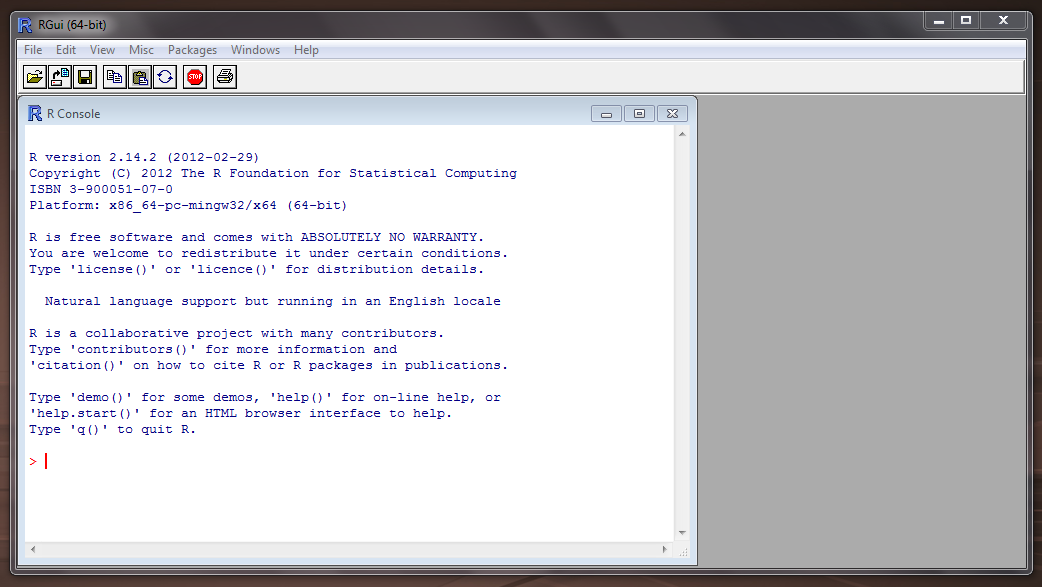
\includegraphics[width=1\linewidth]{images/rgui-windows} \caption{Interface gráfica do usuário no R para Windows.}\label{fig:r-gui}
\end{figure}

\subsubsection{\texorpdfstring{Atualização do no
Windows}{Atualização do  no Windows}}\label{atualizacao-do-no-windows}

Novas versões do R são disponibilizadas em geral com frequência de 5
vezes por ano. Recomenda-se manter o R atualizado, pois as novas versões
incluem
\href{https://cran.r-project.org/bin/windows/base/NEWS.R-3.4.4.html}{aperfeiçoamentos
e a correção de \emph{bugs}}.

As novas versões do vem com os
\href{https://cran.r-project.org/doc/manuals/R-FAQ.html\#Which-add_002don-packages-exist-for-R_003f}{pacotes
padrões do R}. Os demais pacotes instalados pelo usuário na versão
anterior precisam ser reinstalados na nova versão do .

Para atualizar o no Windows, ao invés de baixar o executável a cada nova
versão e repetir o processo da seção anterior, você pode utilizar o
pacote
\href{https://cran.r-project.org/web/packages/installr/index.html}{\textbf{installr}}.
A instalação de pacotes no será vista na seção \ref{install-pck}.

\subsection{Linux}\label{linux}

\subsubsection{Ubuntu}\label{ubuntu}

Há várias formas de instalar o no Ubuntu, mas geralmente a versão
compilada no repositório \emph{default} do Ubuntu não é a última. Se
isso não for problema para você então basta executar:

\begin{Shaded}
\begin{Highlighting}[]
\NormalTok{sudo apt}\OperatorTok{-}\NormalTok{get install r}\OperatorTok{-}\NormalTok{base}
\end{Highlighting}
\end{Shaded}

Entretanto, os pacotes do recém lançados são compilados para última
versão do . Então você pode ter restrições ao uso de pacotes novos, os
quais geralmente incluem o estado da arte de análise de dados. Por esta
razão, abaixo mostra-se como instalar o de forma que seja atualizado
automaticamente pelo sistema.

\subsubsection{R sempre atualizado}\label{r-sempre-atualizado}

Se você quer trabalhar sempre com a última versão estável do , é
possível configurar o Linux Ubuntu para atualizar automaticamente o . O
procedimento de instalação requer senha de superusuário do sistema ou de
privilégios \href{https://en.wikipedia.org/wiki/Sudo}{sudo}. Caso não
tenha, consulte o administrador do sistema.

Ao utilizar distribuições Linux Ubuntu é importante optar por versões
estáveis\footnote{Clique \href{http://releases.ubuntu.com}{aqui} para
  saber mais sobre as versões do Ubuntu.}. As versões de Suporte de
longo prazo (LTS) mais recentes são:

\begin{itemize}
\tightlist
\item
  14.04 (abril de 2014, \emph{codename} \texttt{trusty})
\item
  16.04 (abril de 2016, \emph{codename} \texttt{xenial})
\end{itemize}

A versão mais atual é a R version 3.4.4 (2018-03-15). Para que ele seja
atualizado automaticamente no Ubuntu você precisa adicionar o endereço
do \href{http://cran.r-project.org/mirrors.html}{repósitório do R} mais
próximo de sua região à lista de repositórios do Linux. No exemplo deste
livro, o repositório mais próximo é o da UFPR
(\url{http://cran-r.c3sl.ufpr.br/}).

\paragraph{\texorpdfstring{Incluindo repositório do na Lista de
repositórios do
Ubuntu}{Incluindo repositório do  na Lista de repositórios do Ubuntu}}\label{incluindo-repositorio-do-na-lista-de-repositorios-do-ubuntu}

A lista de repositórios do sistema é armazenada no arquivo
\texttt{/etc/apt/sources.list}. Mas primeiro, você precisa descobrir ou
verificar o nome da versão do sistema operacional. Para isso, você pode
utilizar o seguinte comando\footnote{Se o comando \texttt{lsb\_release}
  não funcionar você precisa instalar o pacote \texttt{lsb-release} no
  sistema. Para isso, digite no terminal Linux
  \texttt{sudo\ apt-get\ install\ lsb-release}.} :

\begin{verbatim}
$ lsb_release --codename | cut -f2
\end{verbatim}

\begin{verbatim}
trusty
\end{verbatim}

Precisamos incluir no arquivo \texttt{sources.list} o espelho do
repositório do R mais próximo. Veja a lista de espelhos de repositórios
do \href{https://cran.r-project.org/mirrors.html}{aqui}. Assim o
gerenciador de pacotes
\href{http://pt.wikipedia.org/wiki/Advanced_Packaging_Tool}{apt}\footnote{o
  gerenciador de pacotes
  \href{http://pt.wikipedia.org/wiki/Advanced_Packaging_Tool}{apt} é
  usado para instalação, atualização e remoção de pacotes em
  distribuições Debian GNU/Linux.} fará a atualização do quando uma nova
versão estiver disponível. Ou seja, você estará utilizando sempre versão
mais atual do .

O endereço do repositório da UFPR será inserido na última linha do
arquivo \texttt{sources.list} usando alguns comandos linux. Essa tarefa
requer privilégios de
\href{https://pt.wikipedia.org/wiki/Superusu\%C3\%A1rio}{superusuário}.
Vamos trocar do seu usuário para o superusuário.

\begin{verbatim}
$ sudo su
\end{verbatim}

Vamos definir no terminal uma variável com o endereço do repositório (da
UFPR nesse caso) e o nome de versão do Ubuntu.

\begin{verbatim}
# repos="deb http://cran-r.c3sl.ufpr.br/bin/linux/ubuntu `lsb_release --codename | cut -f2`/"
\end{verbatim}

Note que a variável \texttt{repos} é uma sequência de caracteres com as
seguintes informações:

\begin{verbatim}
deb `linkRepositorioSelecionado`/bin/linux/ubuntu `versaoUbuntu`/
\end{verbatim}

O valor da variável \texttt{repos} é mostrado pelo comando:
\texttt{echo\ \$repos}. Certifique-se de que a última palavra
corresponde ao nome da sua versão Ubuntu.

Para acrescentar essa informação no final do arquivo
\texttt{sources.list} digite no terminal linux:

\begin{verbatim}
# echo $repos >> /etc/apt/sources.list
\end{verbatim}

Feito isso, você pode retornar a sessão de usuário comum, usando o
comando abaixo:

\begin{verbatim}
# exit
\end{verbatim}

\paragraph{\texorpdfstring{\href{https://cran.r-project.org/bin/linux/ubuntu/README.html\#secure-apt}{APT
protegido}}{APT protegido}}\label{apt-protegido}

Os arquivos binários do para Ubuntu na
\href{http://cran.r-project.org}{CRAN} são assinados com uma chave
pública\footnote{Chave pública de autenticação é um meio alternativo de
  se logar em um servidor ao invés de digitar uma senha. É uma forma
  mais segura e flexível, mas mais difícil de ser configurada. Esse meio
  alternativo de fazer login é importante se o computador está visível
  na internet. Para saber mais veja
  \href{http://the.earth.li/~sgtatham/putty/0.55/htmldoc/Chapter8.html}{aqui}.}
Para adicionar essa chave ao seu sistema digite os seguintes comandos:

\begin{verbatim}
$ gpg --keyserver hkp://keyserver.ubuntu.com:80 --recv-keys E084DAB9
\end{verbatim}

e então use essa informação como entrada no \texttt{apt-key} com

\begin{verbatim}
$ gpg -a --export E084DAB9 | sudo apt-key add -
  
\end{verbatim}

Se aparecer a mensagem de que a chave pública foi importada, então não
há necessidade de executar os comandos abaixo. Mas caso seja impresso
alguma mensagem de erro, outra alternativa pode ser usada para obter a
chave, via os comandos:

\begin{verbatim}
$ gpg --keyserver keyserver.ubuntu.com --recv-key E084DAB9
$ gpg -a --export E084DAB9 | sudo apt-key add -
\end{verbatim}

\paragraph{Atualização da lista de repositórios do Ubuntu e instalação
do
}\label{atualizacao-da-lista-de-repositorios-do-ubuntu-e-instalacao-do}

Após fazer as configurações da lista de repositórios e adicionar a chave
é necessário fazer a atualização dessa lista (requer poderes de super
usuário):

\begin{verbatim}
$ sudo apt-get update
\end{verbatim}

Agora, pode instalar o binário do R:

\begin{verbatim}
$ sudo apt-get install r-base
\end{verbatim}

\paragraph{Testando o }\label{testando-o}

Para iniciar o no Ubuntu, digite \texttt{R} no cursor do terminal:

\begin{verbatim}
$ R
\end{verbatim}

A partir desse momento já começamos uma sessão no . Vamos gerar uma
sequência numérica de 1 a 10 e plotá-la.

\begin{Shaded}
\begin{Highlighting}[]
\OperatorTok{>}\StringTok{ }\DecValTok{1}\OperatorTok{:}\DecValTok{10}
\NormalTok{ [}\DecValTok{1}\NormalTok{]  }\DecValTok{1}  \DecValTok{2}  \DecValTok{3}  \DecValTok{4}  \DecValTok{5}  \DecValTok{6}  \DecValTok{7}  \DecValTok{8}  \DecValTok{9} \DecValTok{10}
\OperatorTok{>}\StringTok{ }\KeywordTok{plot}\NormalTok{(}\DecValTok{1}\OperatorTok{:}\DecValTok{10}\NormalTok{)}
\end{Highlighting}
\end{Shaded}

\begin{figure}

{\centering 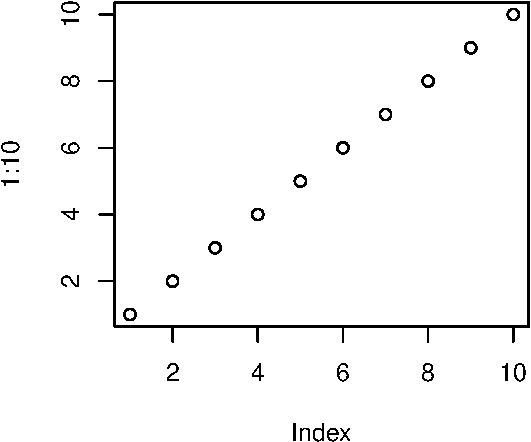
\includegraphics{images/Chunck4-1} 

}

\caption{Gráfico da sequência de 10 números.}\label{fig:Chunck4}
\end{figure}

Você pode sair do , sem salvar os dados da seção, com o código a seguir:

\begin{Shaded}
\begin{Highlighting}[]
\OperatorTok{>}\StringTok{ }\KeywordTok{q}\NormalTok{(}\DataTypeTok{save =} \StringTok{"no"}\NormalTok{)}
\end{Highlighting}
\end{Shaded}

\subsubsection{Diretório para instalação de
pacotes}\label{diretorio-para-instalacao-de-pacotes}

Uma boa prática é definir um diretório para armazenamento dos pacotes
utilizados. Isso lhe dá mais controle sobre os pacotes do instalados no
sistema. Um local sugerido é o \texttt{/home/usuario/.R/libs}. O seu
\texttt{home} ou \texttt{pasta\ pessoal} pode ser obtido com o comando
\texttt{echo\ \$HOME}. Para criar o diretório você pode digitar o
comando abaixo:

\begin{verbatim}
$ mkdir -p `echo $HOME`/.R/libs/
\end{verbatim}

Para informar ao onde procurar os pacotes instalados, você precisa criar
um arquivo chamado \texttt{.Renviron}, no diretório \texttt{\$HOME},
contendo a expressão \texttt{R\_LIBS=/home/usuario/.R/libs/}. Você pode
fazer isso em um terminal com os comandos:

\begin{verbatim}
$ R_LIBS=`echo $HOME/.R/libs/`
$ echo $R_LIBS >> `echo $HOME/.Renviron`
\end{verbatim}

Esse caminho fica então visível ao , o que pode ser verificado
executando a função \texttt{.libPaths()} na linha de comando do .

Abra o :

\begin{verbatim}
$ R
\end{verbatim}

e ao digitar:

\begin{Shaded}
\begin{Highlighting}[]
\OperatorTok{>}\StringTok{ }\KeywordTok{.libPaths}\NormalTok{()}
\NormalTok{[}\DecValTok{1}\NormalTok{] }\StringTok{"/home/pqgfapergs1/.R/libs"}     \StringTok{"/usr/local/lib/R/site-library"}
\NormalTok{[}\DecValTok{3}\NormalTok{] }\StringTok{"/usr/lib/R/site-library"}       \StringTok{"/usr/lib/R/library"}           
\end{Highlighting}
\end{Shaded}

o seu diretório \texttt{/home/usuario/.R/libs}\footnote{Diretórios
  precedidos por ``.'' no Linux são diretórios ocultos. O diretório
  \texttt{/home/usuario/.R} é um diretório oculto, para visualizá-lo no
  Ubuntu, na interface gráfica do sistema, acesse \emph{View
  \textgreater{} Show Hidden Files} (ou \emph{Visualizar \textgreater{}
  Mostrar arquivos ocultos}). No terminal utilize \texttt{ls\ -a} para
  listar os arquivos ocultos.} deve aparecer em primeiro lugar.
Indicando que este local tem prioridade para instalação dos pacotes.
Caso o diretório deixe de existir os seguintes diretórios serão usados.

\section{Pacotes do R}\label{install-pck}

\subsection{Da internet}\label{da-internet}

\subsubsection{CRAN}\label{cran}

A forma mais fácil de instalar uma pacote do R é através da função
\texttt{install.packages("nome\_do\_pacote")}.

Por \emph{default} o pacote informado é instalado a partir da
(\href{https://cran.r-project.org/}{CRAN})

Por exemplo, para instalar o pacote \textbf{devtools}:

\begin{Shaded}
\begin{Highlighting}[]
\KeywordTok{install.packages}\NormalTok{(}\StringTok{"devtools"}\NormalTok{)}
\end{Highlighting}
\end{Shaded}

A função automaticamente resolverá as dependências do pacote, de forma
que qualquer pacote dependente também será instalado.

Para ter acesso as funções disponibilizadas com o pacote você precisa
carregar o pacote:

\begin{Shaded}
\begin{Highlighting}[]
\KeywordTok{library}\NormalTok{(devtools)}
\end{Highlighting}
\end{Shaded}

Para desinstalar um pacote você pode usar a função
\texttt{remove.packages("nome\_do\_pacote")}.

\subsubsection{GitHub e R-forge}\label{github-e-r-forge}

Nem todos pacotes são disponíveis na CRAN. Muitos desenvolvedores
disponibilizam seus pacotes em plataormas como o
\href{https://github.com/}{GitHub} e
\href{https://r-forge.r-project.org/}{R-forge}. As vezes um pacote pode
estar em ambos CRAN e GitHub (ou R-forge), mas a última versão - a de
desenvolvimento - é somente disponibilizada no GitHub (ou R-forge).

Para instalar um pacote de um repositório do GitHub usa-se a função
\texttt{install\_github()} do pacote \textbf{devtools}. Portanto, o
pacote \textbf{devtools} precisa ser instalado primeiro.

Antes de instalar o pacote \textbf{devtools}, usuários Windows precisam
instalar o programa
\href{https://cran.r-project.org/bin/windows/Rtools/index.html}{Rtools}.

A função para instalar um pacote do GitHub requer como argumento o nome
do usuário e do repositório. Por exemplo, para instalar o pacote
\texttt{inmetr} do repositório mantido pelo autor deste livro, usa-se:

\begin{Shaded}
\begin{Highlighting}[]
\CommentTok{# install.packages("devtools")}
\CommentTok{# carrega o pacote devtools}
\KeywordTok{library}\NormalTok{(devtools)}
\CommentTok{# instala o pacote inmetr do repositório }
\CommentTok{# https://github.com/lhmet/inmetr }
\KeywordTok{install_github}\NormalTok{(}\StringTok{"lhmet/inmetr"}\NormalTok{)}
\end{Highlighting}
\end{Shaded}

Para um repositório do R-forge, por exemplo o repositório do pacote
\href{https://r-forge.r-project.org/projects/raster/}{raster}, usa-se:

\begin{Shaded}
\begin{Highlighting}[]
\KeywordTok{install.packages}\NormalTok{(}\StringTok{"raster"}\NormalTok{, }\DataTypeTok{repos =} \StringTok{"http://R-Forge.R-project.org"}\NormalTok{)}
\end{Highlighting}
\end{Shaded}

\subsubsection{Arquivo fonte local}\label{arquivo-fonte-local}

Códigos fonte de pacotes do R são armazenados como arquivos com a
extensão \texttt{.tar.gz}. Binários compilados são armazenados com a
extensão \texttt{.zip}. Exemplo de arquivos como estes podem ser
baixados manualmente da CRAN (veja a seção Downloads em
\url{https://cran.r-project.org/web/packages/ggplot2/index.html}),
GitHub ou R-forge.

Eventualmente um usuário pode instalar um pacote a partir desses
arquivos localmente. Isto pode também ser feito com a função
\texttt{install.packages()}, especifincando o argumento
\texttt{repos\ =\ NULL} e o argumento \texttt{pkgs} com o caminho do
arquivo. Por exemplo:

\begin{Shaded}
\begin{Highlighting}[]
\KeywordTok{install.packages}\NormalTok{(}\StringTok{"ggplot2_2.1.0.tar.gz"}\NormalTok{, }\DataTypeTok{repos=}\OtherTok{NULL}\NormalTok{)}
\end{Highlighting}
\end{Shaded}

\section{RStudio no Ubuntu}\label{install-rstudio}

 é uma empresa que desenvolve ferramentas gratuitas para o e
\href{https://www.rstudio.com/products/}{produtos pagos} para empresas.

Uma de suas ferramentas gratuitas é o software RStudio \emph{Desktop}
que consiste em um ambiente integrado de desenvolvimento
(\href{http://en.wikipedia.org/wiki/Integrated_development_environment}{IDE})
construído especificamente para o , consequentemente, também é
multiplataforma.

Para instalação da versão do RStudio para
\emph{\href{https://pt.wikipedia.org/wiki/Ambiente_de_desktop}{Desktop}},
você precisa saber se seu SO é 64 ou 32-bit e a versão do Linux Ubuntu.
Essas informações podem ser obtidas, respectivamente, pelos comandos:

\begin{verbatim}
$ arch
\end{verbatim}

\begin{verbatim}
x86_64
\end{verbatim}

Se retornar \textbf{x86\_64} sua máquina é 64-bit.

\begin{verbatim}
$ lsb_release --release | cut -f2
\end{verbatim}

\begin{verbatim}
14.04
\end{verbatim}

Com essas informações, siga os seguintes passos:

\begin{enumerate}
\def\labelenumi{\arabic{enumi}.}
\tightlist
\item
  acesse
  \href{https://www.rstudio.com/products/rstudio/download/}{RStudio}
\item
  clique em \emph{Download} (Figura \ref{fig:rstudio-choose})
\end{enumerate}

\begin{figure}

{\centering 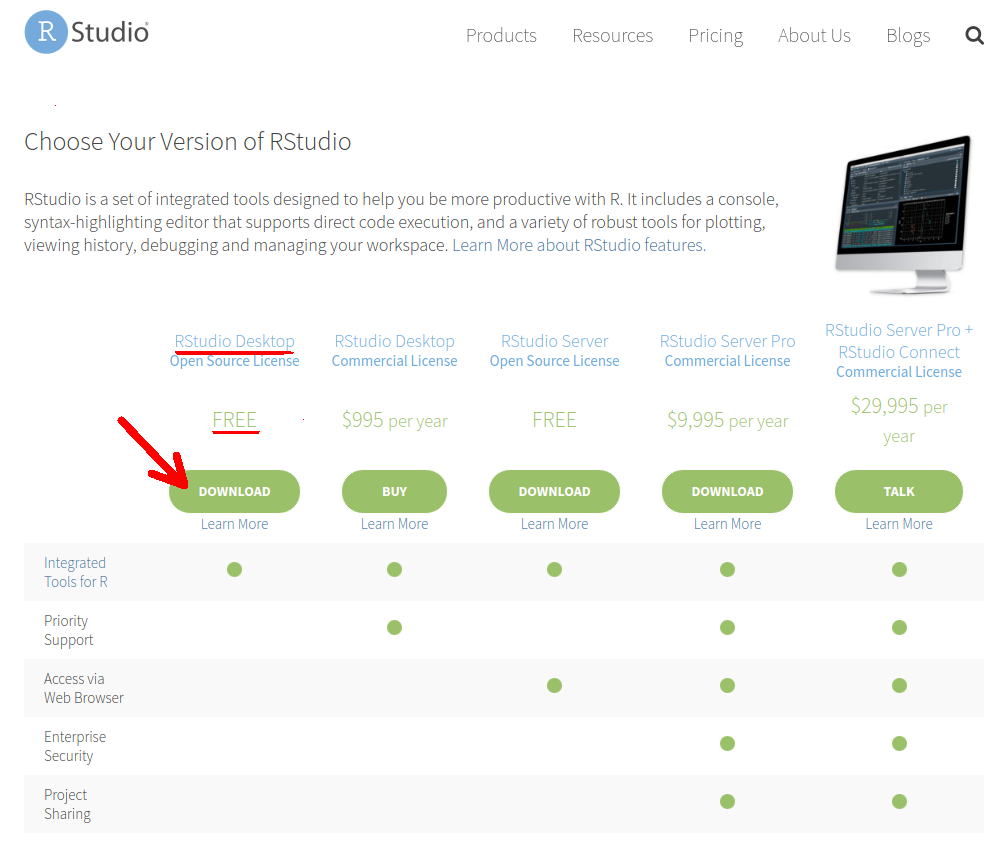
\includegraphics[width=1\linewidth]{images/rstudio-choose} 

}

\caption{Opção para baixar o RStudio *Desktop*.}\label{fig:rstudio-choose}
\end{figure}

\begin{enumerate}
\def\labelenumi{\arabic{enumi}.}
\setcounter{enumi}{2}
\tightlist
\item
  Clique na sua plataforma (de acordo com seu SO, arquitetura e versão
  da distribuição) (Figura \ref{fig:rstudio-plat}), no exemplo deste
  livro \emph{RStudio 1.1.447 - Ubuntu 12.04-15.10/Debian 8 (64-bit)}
\end{enumerate}

\begin{figure}

{\centering 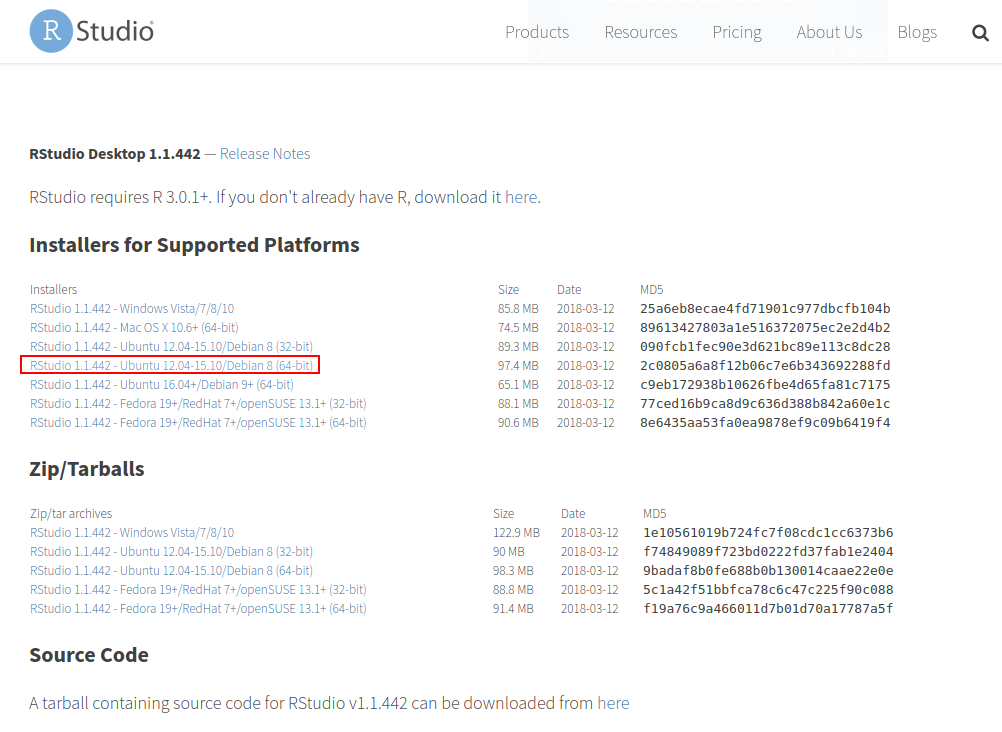
\includegraphics[width=1\linewidth]{images/rstudio-plataform-options} 

}

\caption{Escolha da plataforma em que será o usada o RStudio *Desktop*.}\label{fig:rstudio-plat}
\end{figure}

\begin{enumerate}
\def\labelenumi{\arabic{enumi}.}
\setcounter{enumi}{3}
\tightlist
\item
  Dependendo da sua versão Ubuntu, ao clicar sobre o sobre o arquivo
  baixado com o botão direito, há a opção de abrir com \emph{Ubuntu
  Software Center} e então clicar em \texttt{instalar}. Se na versão de
  seu \emph{Desktop} não há esta opção ao clicar com botão direito sobre
  o arquivo, instale via \textbf{terminal}\footnote{digite `Ctrl+Alt+t'
    para abrir um terminal no Linux Ubuntu} com os seguintes comandos:
\end{enumerate}

\begin{verbatim}
$ cd /local/do/arquivo/baixado
$ sudo dpkg -i arquivoBaixado.deb
$ sudo apt-get install -f
\end{verbatim}

Abra o RStudio digitando no terminal:

\begin{verbatim}
$ rstudio &
\end{verbatim}

Agora você está pronto para começar a programar em aproveitando as
facilidades que o \href{http://www.rstudio.com/}{RStudio} oferece.

\chapter{Interface do Usuário}\label{iu}

Na maior parte do tempo você provavelmente usará o no \textbf{modo
interativo}: rodando comandos e vendo os resultados.

Eventualmente esse processo pode ser inconveniente. Por exemplo, no caso
de uma análise com um código bem extenso e que precisa ser repetida com
dados atualizados semanalmente. Nessa situação, recomenda-se a criação
de um script, ou seja, um arquivo texto, com a extensão \texttt{.R},
contendo o código de sua análise.

Esse \emph{script} pode ser executado pelo R no \textbf{modo de
processamento em lote} (do termo em inglês \emph{Batch Processing})
através de um terminal do SO Linux, ou via o Prompt de comando
(\texttt{cmd.exe}) do SO Windows.

Nesta seção apresenta-se ao leitor estes dois modos de execução do .

\section{ no modo interativo}\label{no-modo-interativo}

No Linux o pode ser aberto simplesmente digitando em um terminal a letra
\texttt{R}.

\begin{Shaded}
\begin{Highlighting}[]
\NormalTok{$ }\ExtensionTok{R}
\end{Highlighting}
\end{Shaded}

\begin{verbatim}
R version 3.4.4 (2018-03-15) -- "Someone to Lean On"
Copyright (C) 2018 The R Foundation for Statistical Computing
Platform: x86_64-pc-linux-gnu (64-bit)

R is free software and comes with ABSOLUTELY NO WARRANTY.
You are welcome to redistribute it under certain conditions.
Type 'license()' or 'licence()' for distribution details.

  Natural language support but running in an English locale

R is a collaborative project with many contributors.
Type 'contributors()' for more information and
'citation()' on how to cite R or R packages in publications.

Type 'demo()' for some demos, 'help()' for on-line help, or
'help.start()' for an HTML browser interface to help.
Type 'q()' to quit R.

> 
\end{verbatim}

A janela com a linha de comando do apresenta o \emph{prompt} do
(\texttt{\textgreater{}}). Após este símbolo digitamos os comandos,
pressionamos a tecla \texttt{\textless{}enter\textgreater{}}, o
interpreta o comando e retorna o resultado.

Os comandos digitados na linha de comando são chamados de expressões.
Esse é o modo iterativo do . Portanto, a linha de comando é a mais
importante ferramenta do , pois todas expressões são avaliadas através
dela.

\begin{Shaded}
\begin{Highlighting}[]
\OperatorTok{>}\StringTok{ }\DecValTok{62} \OperatorTok{+}\StringTok{ }\DecValTok{38}
\NormalTok{[}\DecValTok{1}\NormalTok{] }\DecValTok{100}
\end{Highlighting}
\end{Shaded}

A expressão é avaliada pelo , o resultado é mostrado, mas o seu valor é
perdido.

O número entre colchetes que aparece como resultado da operação
(``{[}1{]}'' no caso acima) indica o conteúdo resultante da operação
iniciando na posição 1 desse objeto. O significado dessa informação
torna-se mais óbvio quando trabalhamos com objetos maiores, como por
exemplo com vetores. Observe os valores nos colchetes para uma sequência
de 100 até 1.

\begin{Shaded}
\begin{Highlighting}[]
\OperatorTok{>}\StringTok{ }\DecValTok{100}\OperatorTok{:}\DecValTok{1}
\NormalTok{  [}\DecValTok{1}\NormalTok{] }\DecValTok{100}  \DecValTok{99}  \DecValTok{98}  \DecValTok{97}  \DecValTok{96}  \DecValTok{95}  \DecValTok{94}  \DecValTok{93}  \DecValTok{92}  \DecValTok{91}  \DecValTok{90}  \DecValTok{89}  \DecValTok{88}  \DecValTok{87}  \DecValTok{86}  \DecValTok{85}  \DecValTok{84}
\NormalTok{ [}\DecValTok{18}\NormalTok{]  }\DecValTok{83}  \DecValTok{82}  \DecValTok{81}  \DecValTok{80}  \DecValTok{79}  \DecValTok{78}  \DecValTok{77}  \DecValTok{76}  \DecValTok{75}  \DecValTok{74}  \DecValTok{73}  \DecValTok{72}  \DecValTok{71}  \DecValTok{70}  \DecValTok{69}  \DecValTok{68}  \DecValTok{67}
\NormalTok{ [}\DecValTok{35}\NormalTok{]  }\DecValTok{66}  \DecValTok{65}  \DecValTok{64}  \DecValTok{63}  \DecValTok{62}  \DecValTok{61}  \DecValTok{60}  \DecValTok{59}  \DecValTok{58}  \DecValTok{57}  \DecValTok{56}  \DecValTok{55}  \DecValTok{54}  \DecValTok{53}  \DecValTok{52}  \DecValTok{51}  \DecValTok{50}
\NormalTok{ [}\DecValTok{52}\NormalTok{]  }\DecValTok{49}  \DecValTok{48}  \DecValTok{47}  \DecValTok{46}  \DecValTok{45}  \DecValTok{44}  \DecValTok{43}  \DecValTok{42}  \DecValTok{41}  \DecValTok{40}  \DecValTok{39}  \DecValTok{38}  \DecValTok{37}  \DecValTok{36}  \DecValTok{35}  \DecValTok{34}  \DecValTok{33}
\NormalTok{ [}\DecValTok{69}\NormalTok{]  }\DecValTok{32}  \DecValTok{31}  \DecValTok{30}  \DecValTok{29}  \DecValTok{28}  \DecValTok{27}  \DecValTok{26}  \DecValTok{25}  \DecValTok{24}  \DecValTok{23}  \DecValTok{22}  \DecValTok{21}  \DecValTok{20}  \DecValTok{19}  \DecValTok{18}  \DecValTok{17}  \DecValTok{16}
\NormalTok{ [}\DecValTok{86}\NormalTok{]  }\DecValTok{15}  \DecValTok{14}  \DecValTok{13}  \DecValTok{12}  \DecValTok{11}  \DecValTok{10}   \DecValTok{9}   \DecValTok{8}   \DecValTok{7}   \DecValTok{6}   \DecValTok{5}   \DecValTok{4}   \DecValTok{3}   \DecValTok{2}   \DecValTok{1}
\end{Highlighting}
\end{Shaded}

O elemento \texttt{{[}18{]}} da sequência de 100 até 1 é o número
\texttt{83}.

Pode ocorrer da expressão digitada na linha ser muito extensa e ir além
de uma linha. Se a expressão estiver incompleta o mostra um sinal de
\texttt{+}.

\begin{Shaded}
\begin{Highlighting}[]
\OperatorTok{>}\StringTok{ }\DecValTok{1} \OperatorTok{*}\StringTok{ }\DecValTok{2} \OperatorTok{*}\StringTok{ }\DecValTok{3} \OperatorTok{*}\StringTok{ }\DecValTok{4} \OperatorTok{*}\StringTok{ }\DecValTok{5} \OperatorTok{*}
\OperatorTok{+}\StringTok{ }\DecValTok{6} \OperatorTok{*}\StringTok{ }\DecValTok{7} \OperatorTok{*}\StringTok{ }\DecValTok{8} \OperatorTok{*}\StringTok{ }\DecValTok{9} \OperatorTok{*}\StringTok{ }\DecValTok{10}
\NormalTok{[}\DecValTok{1}\NormalTok{] }\DecValTok{3628800}
\end{Highlighting}
\end{Shaded}

Execute a expressão abaixo até o sinal de menos e tecle
\texttt{\textless{}enter\textgreater{}}. Enquanto a expressão não
estiver completa o sinal de + se repetirá. Até que você digite o número
que deseja subtrair de 4.

\begin{Shaded}
\begin{Highlighting}[]
\OperatorTok{>}\StringTok{ }\DecValTok{4} \OperatorTok{-}
\OperatorTok{+}\StringTok{   }
\OperatorTok{+}\StringTok{   }\DecValTok{3}
\NormalTok{[}\DecValTok{1}\NormalTok{] }\DecValTok{1}
\end{Highlighting}
\end{Shaded}

\subsection{Expressões em sequência}\label{expressInSeq}

Podemos executar todas expressões anteriores em apenas uma linha, usando
o ponto e vírgula \texttt{;} para separar as expressões:

\begin{Shaded}
\begin{Highlighting}[]
\OperatorTok{>}\StringTok{ }\DecValTok{62} \OperatorTok{+}\StringTok{ }\DecValTok{38}\NormalTok{; }\DecValTok{100}\OperatorTok{:}\DecValTok{1}\NormalTok{; }\DecValTok{1} \OperatorTok{*}\StringTok{ }\DecValTok{2} \OperatorTok{*}\StringTok{ }\DecValTok{3} \OperatorTok{*}\StringTok{ }\DecValTok{4} \OperatorTok{*}\StringTok{ }\DecValTok{5} \OperatorTok{*}\StringTok{ }\DecValTok{6} \OperatorTok{*}\StringTok{ }\DecValTok{7} \OperatorTok{*}\StringTok{ }\DecValTok{8} \OperatorTok{*}\StringTok{ }\DecValTok{9} \OperatorTok{*}\StringTok{ }\DecValTok{10}\NormalTok{; }\DecValTok{4} \OperatorTok{-}\StringTok{ }\DecValTok{3}
\NormalTok{[}\DecValTok{1}\NormalTok{] }\DecValTok{100}
\NormalTok{  [}\DecValTok{1}\NormalTok{] }\DecValTok{100}  \DecValTok{99}  \DecValTok{98}  \DecValTok{97}  \DecValTok{96}  \DecValTok{95}  \DecValTok{94}  \DecValTok{93}  \DecValTok{92}  \DecValTok{91}  \DecValTok{90}  \DecValTok{89}  \DecValTok{88}  \DecValTok{87}  \DecValTok{86}  \DecValTok{85}  \DecValTok{84}
\NormalTok{ [}\DecValTok{18}\NormalTok{]  }\DecValTok{83}  \DecValTok{82}  \DecValTok{81}  \DecValTok{80}  \DecValTok{79}  \DecValTok{78}  \DecValTok{77}  \DecValTok{76}  \DecValTok{75}  \DecValTok{74}  \DecValTok{73}  \DecValTok{72}  \DecValTok{71}  \DecValTok{70}  \DecValTok{69}  \DecValTok{68}  \DecValTok{67}
\NormalTok{ [}\DecValTok{35}\NormalTok{]  }\DecValTok{66}  \DecValTok{65}  \DecValTok{64}  \DecValTok{63}  \DecValTok{62}  \DecValTok{61}  \DecValTok{60}  \DecValTok{59}  \DecValTok{58}  \DecValTok{57}  \DecValTok{56}  \DecValTok{55}  \DecValTok{54}  \DecValTok{53}  \DecValTok{52}  \DecValTok{51}  \DecValTok{50}
\NormalTok{ [}\DecValTok{52}\NormalTok{]  }\DecValTok{49}  \DecValTok{48}  \DecValTok{47}  \DecValTok{46}  \DecValTok{45}  \DecValTok{44}  \DecValTok{43}  \DecValTok{42}  \DecValTok{41}  \DecValTok{40}  \DecValTok{39}  \DecValTok{38}  \DecValTok{37}  \DecValTok{36}  \DecValTok{35}  \DecValTok{34}  \DecValTok{33}
\NormalTok{ [}\DecValTok{69}\NormalTok{]  }\DecValTok{32}  \DecValTok{31}  \DecValTok{30}  \DecValTok{29}  \DecValTok{28}  \DecValTok{27}  \DecValTok{26}  \DecValTok{25}  \DecValTok{24}  \DecValTok{23}  \DecValTok{22}  \DecValTok{21}  \DecValTok{20}  \DecValTok{19}  \DecValTok{18}  \DecValTok{17}  \DecValTok{16}
\NormalTok{ [}\DecValTok{86}\NormalTok{]  }\DecValTok{15}  \DecValTok{14}  \DecValTok{13}  \DecValTok{12}  \DecValTok{11}  \DecValTok{10}   \DecValTok{9}   \DecValTok{8}   \DecValTok{7}   \DecValTok{6}   \DecValTok{5}   \DecValTok{4}   \DecValTok{3}   \DecValTok{2}   \DecValTok{1}
\NormalTok{[}\DecValTok{1}\NormalTok{] }\DecValTok{3628800}
\NormalTok{[}\DecValTok{1}\NormalTok{] }\DecValTok{1}
\end{Highlighting}
\end{Shaded}

\subsection{Navegação entre as expressões já
avaliadas}\label{navegacao-entre-as-expressoes-ja-avaliadas}

Você pode usar as teclas ⬆️ e ⬇️ para navegar entre as expressões já
avaliadas pelo . O que é útil quando precisamos repetir um comando
anterior com alguma mudança ou para corrigir um erro de digitação ou a
omissão de um parentêses.

Quando a linha de comando é usada por muito tempo a sua tela pode ficar
poluída com a saída das expressões anteriores. Para limpar a tela, tecle
\texttt{Ctrl+l}. Assim o console aparece na parte superior do terminal.

\begin{Shaded}
\begin{Highlighting}[]
\OperatorTok{>}\StringTok{ }\DecValTok{15} \OperatorTok{+}\StringTok{ }\DecValTok{4}
\NormalTok{[}\DecValTok{1}\NormalTok{] }\DecValTok{19}
\OperatorTok{>}\StringTok{ }\DecValTok{100}\OperatorTok{:}\DecValTok{1}
\NormalTok{  [}\DecValTok{1}\NormalTok{] }\DecValTok{100}  \DecValTok{99}  \DecValTok{98}  \DecValTok{97}  \DecValTok{96}  \DecValTok{95}  \DecValTok{94}  \DecValTok{93}  \DecValTok{92}  \DecValTok{91}  \DecValTok{90}  \DecValTok{89}  \DecValTok{88}  \DecValTok{87}  \DecValTok{86}  \DecValTok{85}  \DecValTok{84}
\NormalTok{ [}\DecValTok{18}\NormalTok{]  }\DecValTok{83}  \DecValTok{82}  \DecValTok{81}  \DecValTok{80}  \DecValTok{79}  \DecValTok{78}  \DecValTok{77}  \DecValTok{76}  \DecValTok{75}  \DecValTok{74}  \DecValTok{73}  \DecValTok{72}  \DecValTok{71}  \DecValTok{70}  \DecValTok{69}  \DecValTok{68}  \DecValTok{67}
\NormalTok{ [}\DecValTok{35}\NormalTok{]  }\DecValTok{66}  \DecValTok{65}  \DecValTok{64}  \DecValTok{63}  \DecValTok{62}  \DecValTok{61}  \DecValTok{60}  \DecValTok{59}  \DecValTok{58}  \DecValTok{57}  \DecValTok{56}  \DecValTok{55}  \DecValTok{54}  \DecValTok{53}  \DecValTok{52}  \DecValTok{51}  \DecValTok{50}
\NormalTok{ [}\DecValTok{52}\NormalTok{]  }\DecValTok{49}  \DecValTok{48}  \DecValTok{47}  \DecValTok{46}  \DecValTok{45}  \DecValTok{44}  \DecValTok{43}  \DecValTok{42}  \DecValTok{41}  \DecValTok{40}  \DecValTok{39}  \DecValTok{38}  \DecValTok{37}  \DecValTok{36}  \DecValTok{35}  \DecValTok{34}  \DecValTok{33}
\NormalTok{ [}\DecValTok{69}\NormalTok{]  }\DecValTok{32}  \DecValTok{31}  \DecValTok{30}  \DecValTok{29}  \DecValTok{28}  \DecValTok{27}  \DecValTok{26}  \DecValTok{25}  \DecValTok{24}  \DecValTok{23}  \DecValTok{22}  \DecValTok{21}  \DecValTok{20}  \DecValTok{19}  \DecValTok{18}  \DecValTok{17}  \DecValTok{16}
\NormalTok{ [}\DecValTok{86}\NormalTok{]  }\DecValTok{15}  \DecValTok{14}  \DecValTok{13}  \DecValTok{12}  \DecValTok{11}  \DecValTok{10}   \DecValTok{9}   \DecValTok{8}   \DecValTok{7}   \DecValTok{6}   \DecValTok{5}   \DecValTok{4}   \DecValTok{3}   \DecValTok{2}   \DecValTok{1}
\OperatorTok{>}\StringTok{ }\CommentTok{#tecle <Ctr + l>}
\end{Highlighting}
\end{Shaded}

Para parar ou cancelar a execução de uma expressão utilize as teclas
\texttt{Ctrl\ +\ C}. As teclas \texttt{Ctrl\ +\ l} tem o efeito de
limpar a tela.

\subsection{Comentários}\label{comentarios}

No , a cerquilha \texttt{\#} (hashtag) é um caracter especial. Qualquer
coisa após esse caracter será ignorada pelo . Somente as expressões
antes da \texttt{\#} são avaliadas. Por meio desse símbolo de comentário
podemos fazer anotações e comentários no código sem atrapalhar a
interpretação das expressões pelo .

\begin{Shaded}
\begin{Highlighting}[]
\OperatorTok{>}\StringTok{ }\CommentTok{# comentário antes do código }
\end{Highlighting}
\end{Shaded}

\begin{Shaded}
\begin{Highlighting}[]
\OperatorTok{>}\StringTok{ }\DecValTok{17} \OperatorTok{+}\StringTok{ }\DecValTok{3} \CommentTok{# comentário ao lado do código: adicionando 17 e 3}
\NormalTok{[}\DecValTok{1}\NormalTok{] }\DecValTok{20}
\end{Highlighting}
\end{Shaded}

\subsection{Auto preenchimento de
funções}\label{auto-preenchimento-de-funcoes}

O inclui o preenchimento automático de nomes de funções e arquivos por
meio da tecla \texttt{\textless{}tab\textgreater{}}. Uma lista de
possíveis funções que começam com as letras inicialmente digitadas
aparecerão.

\begin{Shaded}
\begin{Highlighting}[]
\OperatorTok{>}\StringTok{ }\NormalTok{read}\CommentTok{#<tab> pressione <tab> para ver as opções de comandos que iniciam com o termo read}
\end{Highlighting}
\end{Shaded}

\subsection{\texorpdfstring{Primeiro
\emph{script}}{Primeiro script}}\label{primeiro-script}

O trecho de código abaixo apresenta nas primeiras linhas algumas
expressões do executadas anteriormente. Mas há também, na segunda parte,
códigos para salvar um gráfico de pontos num arquivo \emph{pdf}. Na
última parte do trecho, define-se uma variável \texttt{x} que contém
aquela mesma sequência numérica usada no gráfico.

\begin{Shaded}
\begin{Highlighting}[]
\CommentTok{# Primeiro script no R}
\CommentTok{#----------------------------------------------------------------}
\CommentTok{# cálculos básicos}
\DecValTok{15} \OperatorTok{+}\StringTok{ }\DecValTok{4}
\DecValTok{1}\OperatorTok{:}\DecValTok{100}
\DecValTok{1} \OperatorTok{*}\StringTok{ }\DecValTok{2} \OperatorTok{*}\StringTok{ }\DecValTok{3} \OperatorTok{*}\StringTok{ }\DecValTok{4} \OperatorTok{*}\StringTok{ }\DecValTok{5} \OperatorTok{*}\DecValTok{6} \OperatorTok{*}\StringTok{ }\DecValTok{7} \OperatorTok{*}\StringTok{ }\DecValTok{8} \OperatorTok{*}\StringTok{ }\DecValTok{9} \OperatorTok{*}\StringTok{ }\DecValTok{10}
\DecValTok{4}\OperatorTok{-}\DecValTok{3}
\CommentTok{#----------------------------------------------------------------}
\CommentTok{# salvando um gráfico em um arquivo pdf}
\NormalTok{arquivo_pdf <-}\StringTok{ "plot-script1.pdf"}
\KeywordTok{pdf}\NormalTok{(arquivo_pdf)        }\CommentTok{# cria e abre um arquivo pdf}
\KeywordTok{plot}\NormalTok{(}\DecValTok{1}\OperatorTok{:}\DecValTok{100}\NormalTok{)             }\CommentTok{# faz o gráfico}
\KeywordTok{dev.off}\NormalTok{()               }\CommentTok{# fecha o arquivo pdf}
\CommentTok{#----------------------------------------------------------------}
\CommentTok{# definindo uma variável x}
\NormalTok{x <-}\StringTok{ }\DecValTok{1}\OperatorTok{:}\DecValTok{100}
\NormalTok{x}
\end{Highlighting}
\end{Shaded}

Este conjunto de linhas de código, quando inseridos em um arquivo
texto\footnote{Para fazer isso, você pode usar um editor de texto
  qualquer (p.ex.:
  \href{https://help.gnome.org/users/gedit/stable/index.html.pt_BR}{gedit}
  no SO Linux, ou
  \href{https://pt.wikipedia.org/wiki/Bloco_de_Notas}{Notepad} no SO
  Windows).} formam um primeiro \emph{script} . Este \emph{script} pode
ser executado pelo através da função \texttt{source()}, usando como
argumento o caminho para o local do \emph{script}.

\begin{Shaded}
\begin{Highlighting}[]
\OperatorTok{>}\StringTok{ }\KeywordTok{source}\NormalTok{(}\StringTok{"/home/usuario/adar/script1.R"}\NormalTok{)}
\end{Highlighting}
\end{Shaded}

Este \emph{script} produzirá como saída o arquivo
\texttt{/home/usuario/adar/plot-script1.pdf}. Você pode visualizar o
arquivo para conferir o gráficos de pontos gerado.

\section{ no modo de processamento em
lote}\label{no-modo-de-processamento-em-lote}

Para rodar um \emph{script} no modo de processamento em lote do através
do seguinte comando no terminal Linux:

\begin{verbatim}
$ R CMD BATCH opcoes arqentrada arqsaida
\end{verbatim}

Onde: \texttt{arqentrada}é o nome do script (arquivo com a extensão
\texttt{.R}) a ser executado; \texttt{arqsaida} é o arquivo (com a
extensão \texttt{.Rout}) com as saídas dos comandos executados no R;
\texttt{opcoes} é a lista de opções que controlam a execução.

Vamos rodar como exemplo, o \texttt{script1.R} da seção
\ref{primeiro-script}.

\begin{verbatim}
$ R CMD BATCH /home/usuario/adar/script1.R
\end{verbatim}

O comando acima, produzirá dois arquivos de saída:

\begin{enumerate}
\def\labelenumi{\arabic{enumi}.}
\tightlist
\item
  \texttt{script1.Rout}\footnote{Você pode notar que este arquivo tem o
    mesmo nome do \texttt{arqentrada}, exceto que a sua extensão foi
    alterada para \texttt{.Rout}.} criado por \emph{default} quando o
  \texttt{arqsaida} não é especificado, e;
\end{enumerate}

\begin{enumerate}
\def\labelenumi{\arabic{enumi}.}
\setcounter{enumi}{1}
\tightlist
\item
  arquivo "plot-script1.pdf".
\end{enumerate}

Você pode especificar o nome do \texttt{arqsaida} como desejar. No
exemplo abaixo, mostra-se como salvar o arquivo de saída incluindo a
data em que ele foi gerado, \texttt{script1-saida-adatadehoje.log}.

\begin{verbatim}
$ R CMD BATCH script1.R script1-saida-`date "+%Y%m%d"`.log
\end{verbatim}

Após a execução do último comando, os mesmos arquivos resultantes do
comando anterior serão gerados, exceto pelo primeiro (\texttt{.Rout}),
que será nomeado \texttt{script1-saida-20180423.Rout}.

Para mais opções do comando \texttt{R\ CMD\ BATCH} digite no terminal do
Linux \texttt{R\ -\/-help}.

\chapter{RStudio}\label{rstudio}

O RStudio \emph{Desktop} é um ambiente integrado de desenvolvimento
(IDE) para o . Portanto, o RStudio depende da instalação prévia do . Ele
funciona como uma interface gráfica do usuário (GUI), mas com muito mais
potencialidades.

O RStudio é uma ferramente que potencializará sua interação com o :

\begin{itemize}
\item
  na produção de gráficos
\item
  na organização de seu código na forma de projetos
\item
  na reprodutibilidade de seu trabalho ou pesquisa
\item
  na manutenção e criação de seus próprios pacotes do R
\item
  na criação e compartilhamento de seus relatórios
\item
  no compartilhamento de seu código e a colaboração com outros
\end{itemize}

Nessa seção você terá uma visão geral do RStudio \emph{Desktop}.

\section{Visão geral do RStudio}\label{visao-geral-do-rstudio}

Assumindo que o RStudio tenha sido instalado (seção
\ref{install-rstudio}), ao abri-lo e clicar em \emph{File \textgreater{}
New File \textgreater{} R script} você verá uma tela com aspecto similar
ao da Figura \ref{fig:rstudio-fig}.

\begin{figure}
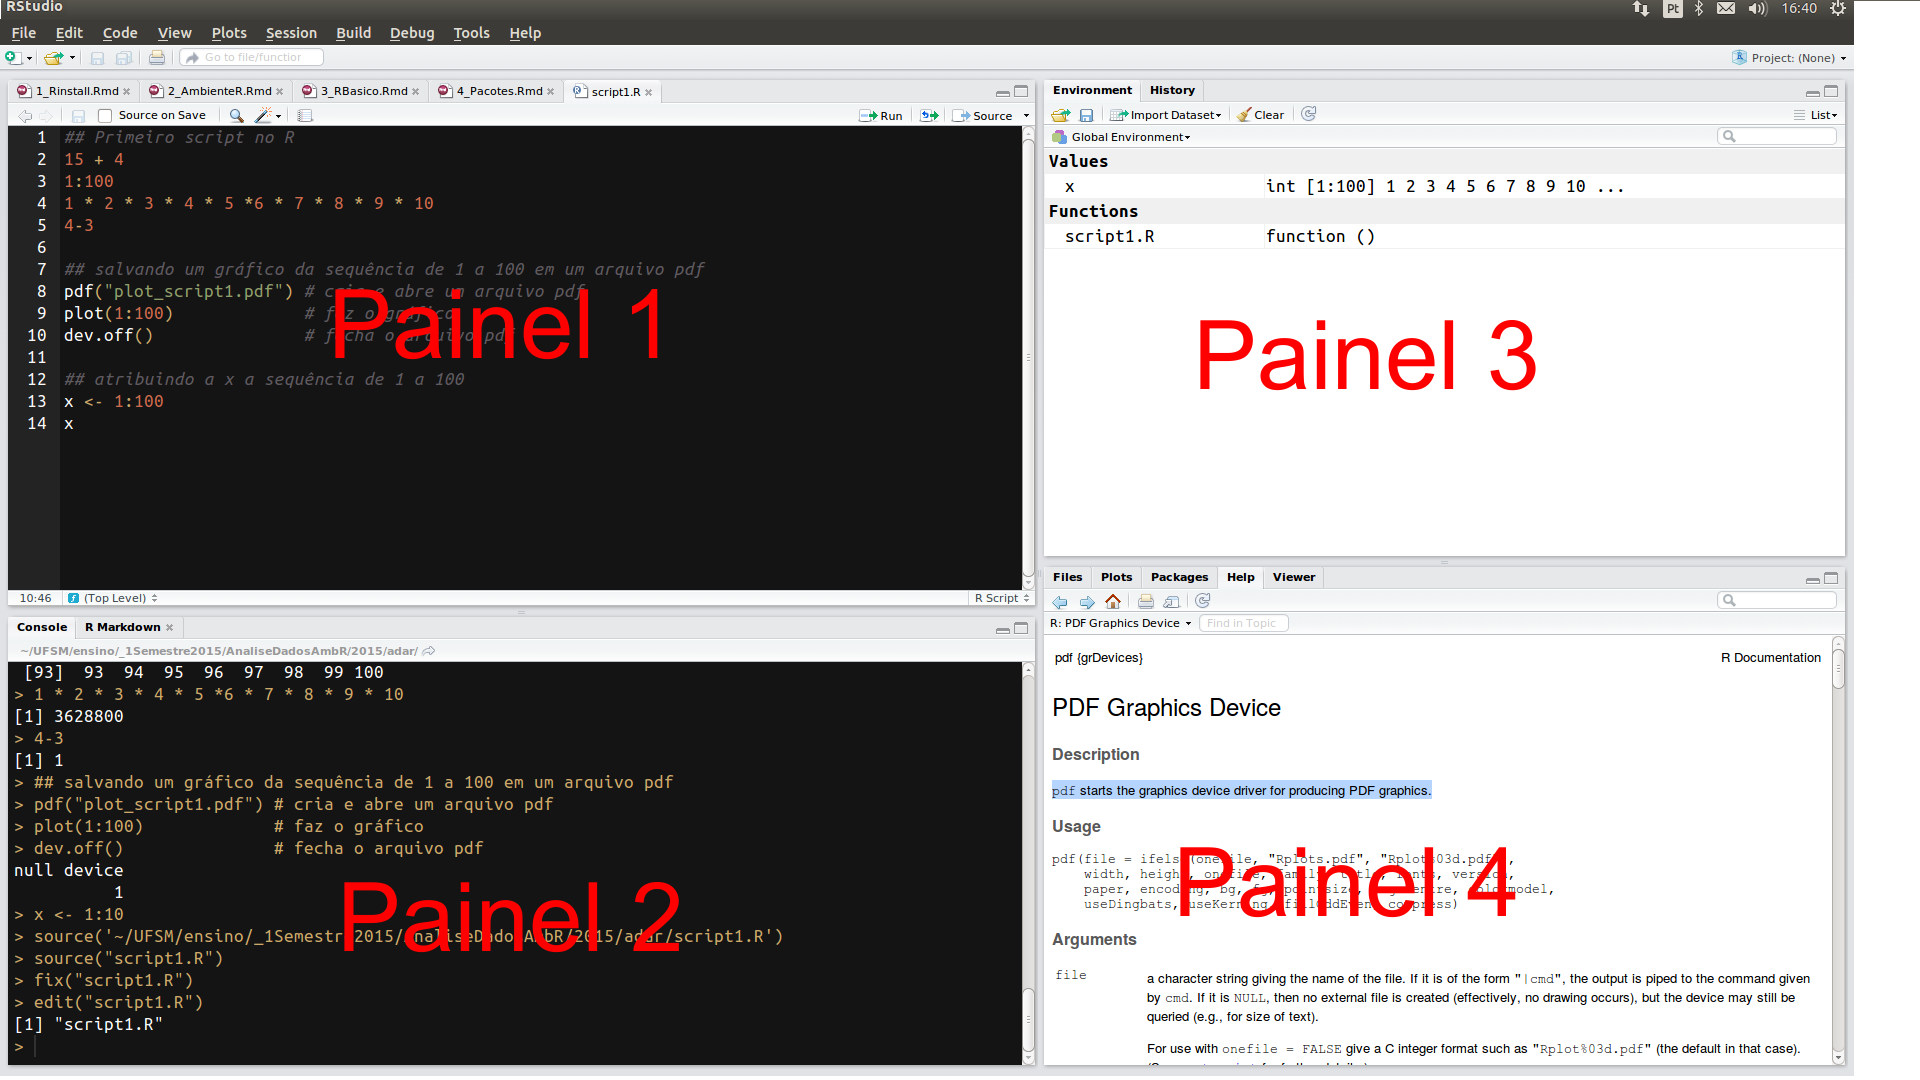
\includegraphics[width=26.67in]{images/Rstudio_panels} \caption{Rstudio}\label{fig:rstudio-fig}
\end{figure}

O RStudio possui 4 painéis principais:

\begin{enumerate}
\def\labelenumi{\arabic{enumi}.}
\item
  Editor para scripts e visualização de dados

  \begin{itemize}
  \tightlist
  \item
    abrir e criar scripts
  \item
    rodar scripts
  \item
    código com sintaxe realçada
  \item
    rodar partes do código \texttt{\textless{}Ctrl+enter\textgreater{}}
  \item
    rodar todo script \texttt{\textless{}Ctrl+Shift+S\textgreater{}}
  \item
    autopreenchimento das funções \texttt{\textless{}tab\textgreater{}}
  \item
    comentar linhas \texttt{\textless{}Ctrl+Shift+C\textgreater{}}
  \item
    desfazer \texttt{\textless{}Ctrl+Z\textgreater{}}
  \item
    refazer \texttt{\textless{}Ctrl+Shift+Z\textgreater{}}
  \item
    referência para teclas de atalho
    \texttt{\textless{}Alt+Shift+K\textgreater{}}
  \item
    abrir script com \texttt{\textless{}Ctrl+Click\textgreater{}}
  \item
    encontrar e substituir \texttt{Ctrl+F}
  \end{itemize}
\item
  Console do R
\item
  Navegador do espaço de trabalho e histórico de comandos
\item
  Arquivos/Plots/Pacotes/Ajuda/Visualizador
\end{enumerate}

Configuração de texto e painéis em:

\begin{itemize}
\tightlist
\item
  Menus

  \begin{itemize}
  \tightlist
  \item
    Tools \textgreater{} global Options \textgreater{} Appearance

    \begin{itemize}
    \tightlist
    \item
      mostrar linhas, alterar realce da sintaxe
    \end{itemize}
  \item
    Session
  \item
    Plots
  \end{itemize}
\end{itemize}

Para saber mais sobre os recursos fornecidos pelo RStudio assista ao
vídeo
\emph{\href{https://www.rstudio.com/resources/webinars/rstudio-essentials-webinar-series-part-1/}{RStudio
Essencials}}. Isso o ajudará a usar mais efetivamente o RStudio.

\textbf{Folha de referência do RStudio}

\begin{figure}

{\centering 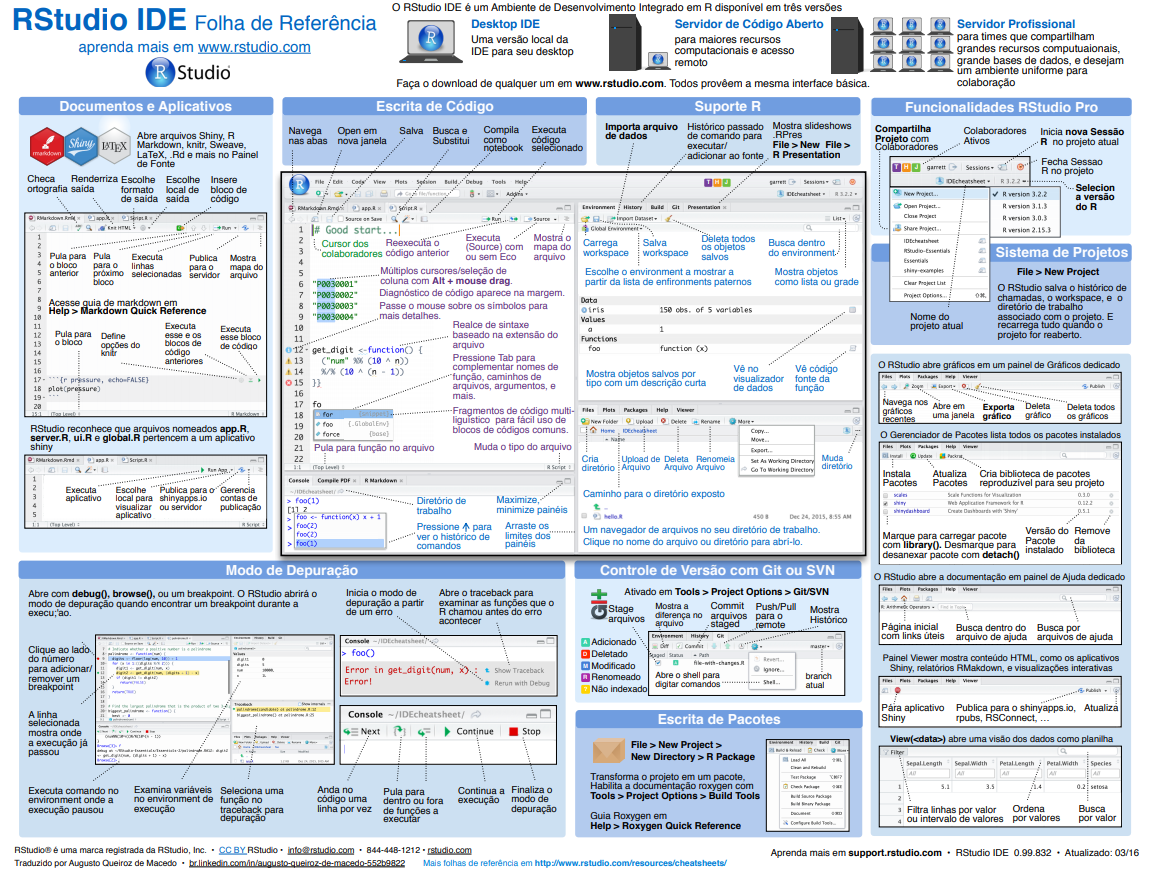
\includegraphics[width=1\linewidth]{images/print-screen-folha-ref-rstudio} 

}

\caption{Folha de referência do RStudio, disponível em https://www.rstudio.com/wp-content/uploads/2016/03/rstudio-IDE-cheatsheet-portuguese.pdf}\label{fig:cheat-sheet}
\end{figure}

\chapter{Operações básicas}\label{operbasic}

Nesta seção veremos:

\begin{itemize}
\tightlist
\item
  operações aritméticas básicas com R
\item
  a atribuição de valores a uma variável
\item
  o uso de funções matemáticas internas do R
\item
  valores numéricos especiais do R
\item
  os cuidados ao nomear variáveis
\end{itemize}

\section{Convenção}\label{convencao}

A partir deste capítulo, os códigos a serem avaliadas no {R} terão o
prompt do {R} (\texttt{\textgreater{}}) omitidos. Essa convenção é para
tornar mais fácil a ação de copiar e colar os códigos na linha de
comando do {R}. O resultado da avaliação das expressões será mostrado
precedido do símbolo (\texttt{\#\textgreater{}}). Esses valores são os
resultados que esperam-se sejam reproduzidos pelo leitor na sessão do
{R} em seu computador. Por exemplo:

\begin{Shaded}
\begin{Highlighting}[]
\DecValTok{1}\OperatorTok{:}\DecValTok{5}
\CommentTok{#> [1] 1 2 3 4 5}
\end{Highlighting}
\end{Shaded}

No trecho de código acima, a primeira linha contém o código a ser
copiado pelo leitor para execução em seu computador. A segunda linha é a
saída do código avaliado pelo R.

\section{Calculadora}\label{calculadora}

O R é uma calculadora turbinada com diversas funções matemáticas
disponíveis. Para quem não conhece o R, essa uma forma de
familiarizar-se com a linha de comandos do R.

\subsection{Aritmética básica}\label{aritmetica-basica}

Todas operações feitas em uma calculadora podem ser realizadas na linha
de comandos do R.

\begin{Shaded}
\begin{Highlighting}[]
\DecValTok{10} \OperatorTok{+}\StringTok{ }\DecValTok{2} \OperatorTok{+}\StringTok{ }\DecValTok{4}
\CommentTok{#> [1] 16}
\CommentTok{# Exemplo de divisao }
\NormalTok{(}\DecValTok{5} \OperatorTok{+}\StringTok{ }\DecValTok{14}\NormalTok{)}\OperatorTok{/}\DecValTok{2}
\CommentTok{#> [1] 9.5}
\CommentTok{# exponenciação}
\DecValTok{2}\OperatorTok{^}\DecValTok{3}
\CommentTok{#> [1] 8}
\DecValTok{4}\OperatorTok{^}\FloatTok{0.5}
\CommentTok{#> [1] 2}
\CommentTok{# operador artimético para se determinar o resto de uma divisao}
\DecValTok{10} \OperatorTok\StringTok{ }\DecValTok{2}
\CommentTok{#> [1] 0}
\DecValTok{2001} \OperatorTok\StringTok{ }\DecValTok{2}
\CommentTok{#> [1] 1}
\CommentTok{# o inteiro do quociente }
\DecValTok{11} \OperatorTok\StringTok{ }\DecValTok{2}
\CommentTok{#> [1] 5}
\end{Highlighting}
\end{Shaded}

\begin{rmdwarning}
Note que no R, o separador decimal é o ponto ".", ao invés da vírgula
"," usada na notação brasileira. As vírgulas tem a finalidade de separar
os argumentos nas chamadas de funções, tal como em
\texttt{log(x\ =\ 10,\ base\ =\ 10)}.
\end{rmdwarning}

Conheça mais operadores aritméticos, digitando na linha de comando:

\begin{Shaded}
\begin{Highlighting}[]
\NormalTok{?}\StringTok{"Arithmetic"}
\end{Highlighting}
\end{Shaded}

A janela que se abrirá mostrará o texto que faz parte do manual de ajuda
do {R}.

\subsection{Constantes}\label{constantes}

O R possui algumas constantes pré-definidas, como o a constante pi
(\(\pi\)).

\begin{Shaded}
\begin{Highlighting}[]
\NormalTok{pi}
\CommentTok{#> [1] 3.141593}
\end{Highlighting}
\end{Shaded}

O R também tem vetores de caracteres pré-definidos, são eles:

\begin{Shaded}
\begin{Highlighting}[]
\NormalTok{LETTERS}
\CommentTok{#>  [1] "A" "B" "C" "D" "E" "F" "G" "H" "I" "J" "K" "L" "M" "N" "O" "P" "Q"}
\CommentTok{#> [18] "R" "S" "T" "U" "V" "W" "X" "Y" "Z"}
\NormalTok{letters}
\CommentTok{#>  [1] "a" "b" "c" "d" "e" "f" "g" "h" "i" "j" "k" "l" "m" "n" "o" "p" "q"}
\CommentTok{#> [18] "r" "s" "t" "u" "v" "w" "x" "y" "z"}
\NormalTok{month.abb}
\CommentTok{#>  [1] "Jan" "Feb" "Mar" "Apr" "May" "Jun" "Jul" "Aug" "Sep" "Oct" "Nov"}
\CommentTok{#> [12] "Dec"}
\NormalTok{month.name}
\CommentTok{#>  [1] "January"   "February"  "March"     "April"     "May"      }
\CommentTok{#>  [6] "June"      "July"      "August"    "September" "October"  }
\CommentTok{#> [11] "November"  "December"}
\end{Highlighting}
\end{Shaded}

Note que caracteres estão sempre entre aspas: \texttt{""}.

``caracteres são entre aspas''

\begin{Shaded}
\begin{Highlighting}[]
\NormalTok{aeiou}
\CommentTok{#> Error in eval(expr, envir, enclos): object 'aeiou' not found}
\end{Highlighting}
\end{Shaded}

\begin{Shaded}
\begin{Highlighting}[]
\StringTok{"aeiou"}
\CommentTok{#> [1] "aeiou"}
\end{Highlighting}
\end{Shaded}

\subsection{Funções matemáticas
internas}\label{funcoes-matematicas-internas}

Existem diversas funções internas do R que permitem, por exemplo,
sortear números aleatóriamente, arrendondar números, calcular o
fatorial, calcular o seno, cosseno de um ângulo e etc. A sintaxe para
chamar uma função no R é:

\texttt{funcão(argumento)}

Por exemplo:

\begin{Shaded}
\begin{Highlighting}[]
\CommentTok{# funções trigonométricas}
\KeywordTok{sin}\NormalTok{(pi}\OperatorTok{/}\DecValTok{6}\NormalTok{)}
\CommentTok{#> [1] 0.5}
\KeywordTok{cos}\NormalTok{(pi)}
\CommentTok{#> [1] -1}
\CommentTok{# raiz quadrada}
\KeywordTok{sqrt}\NormalTok{(}\DecValTok{100}\NormalTok{)}
\CommentTok{#> [1] 10}
\CommentTok{# exponencial}
\KeywordTok{exp}\NormalTok{(}\DecValTok{1}\NormalTok{)}
\CommentTok{#> [1] 2.718282}
\CommentTok{# fatorial}
\KeywordTok{factorial}\NormalTok{(}\DecValTok{4}\NormalTok{)}
\CommentTok{#> [1] 24}
\end{Highlighting}
\end{Shaded}

No R você verá que parênteses são frequentemente utilizados. Eles são
sempre associados à funções. Qualquer palavra antecedendo um parênteses
é uma função.

Para ver a lista completa de funções trigonométricas:

\begin{Shaded}
\begin{Highlighting}[]
\NormalTok{?}\StringTok{"Trig"}
\end{Highlighting}
\end{Shaded}

\subsection{Valores numéricos
especiais}\label{valores-numericos-especiais}

Um caso particular sobre operação aritméticas no R, são os valores
numéricos \texttt{Inf}e \texttt{NaN} que resultam de operações como:

\begin{Shaded}
\begin{Highlighting}[]
\DecValTok{2}\OperatorTok{/}\DecValTok{0}
\CommentTok{#> [1] Inf}
\OperatorTok{-}\DecValTok{12}\OperatorTok{/}\DecValTok{0}
\CommentTok{#> [1] -Inf}
\KeywordTok{exp}\NormalTok{(}\OperatorTok{-}\OtherTok{Inf}\NormalTok{)}
\CommentTok{#> [1] 0}
\KeywordTok{log}\NormalTok{(}\DecValTok{0}\NormalTok{)}
\CommentTok{#> [1] -Inf}
\DecValTok{0}\OperatorTok{/}\OtherTok{Inf}
\CommentTok{#> [1] 0}
\NormalTok{(}\DecValTok{0}\OperatorTok{:}\DecValTok{3}\NormalTok{)}\OperatorTok{^}\OtherTok{Inf}
\CommentTok{#> [1]   0   1 Inf Inf}
\KeywordTok{log}\NormalTok{(}\OperatorTok{-}\FloatTok{0.5}\NormalTok{)}
\CommentTok{#> Warning in log(-0.5): NaNs produced}
\CommentTok{#> [1] NaN}
\KeywordTok{sqrt}\NormalTok{(}\OperatorTok{-}\DecValTok{1}\NormalTok{)}
\CommentTok{#> Warning in sqrt(-1): NaNs produced}
\CommentTok{#> [1] NaN}
\DecValTok{0}\OperatorTok{/}\DecValTok{0} 
\CommentTok{#> [1] NaN}
\OtherTok{Inf}\OperatorTok{-}\OtherTok{Inf}
\CommentTok{#> [1] NaN}
\OtherTok{Inf}\OperatorTok{/}\OtherTok{Inf}
\CommentTok{#> [1] NaN}
\KeywordTok{mean}\NormalTok{(}\KeywordTok{c}\NormalTok{(}\OtherTok{NA}\NormalTok{, }\OtherTok{NA}\NormalTok{), }\DataTypeTok{na.rm =} \OtherTok{TRUE}\NormalTok{)}
\CommentTok{#> [1] NaN}
\end{Highlighting}
\end{Shaded}

\texttt{NaN} é a abreviação para \emph{Not a Number}. Geralmente surge
quando um cálculo não tem sentido matemático ou não pode ser
propriamente realizado.

A demonstração das diferentes formas de se obter essas constantes
especiais é importante para entender a origem delas durante a execução
de um script mais extenso.

Outra constante especial do R é o \texttt{NA} (\emph{Not Available}) que
representa valor faltante, um problema comum em análise de dados.
Qualquer operação envolvendo \texttt{NA} resultará em \texttt{NA}
(Tabela 1).

\begin{table}

\caption{\label{tab:chunk19}Tabela 1. Operações com NA.}
\centering
\begin{tabular}[t]{c|c}
\hline
operação & resultado\\
\hline
NA + 5 & NA\\
\hline
sqrt(NA) & NA\\
\hline
NA\textasciicircum{}2 & NA\\
\hline
NA/NaN & NA\\
\hline
\end{tabular}
\end{table}

\subsection{Notação científica e número de
dígitos}\label{notacao-cientifica-e-numero-de-digitos}

Na maioria das vezes precisamos trabalhar com números grandes e
consequentemente acabamos usando uma notação científica ou exponencial.
No R há diferentes formas de representar números com expoentes:

\begin{Shaded}
\begin{Highlighting}[]
\FloatTok{1.2e-6}
\CommentTok{#> [1] 1.2e-06}
\CommentTok{# expressões equivalentes}
\FloatTok{1.2E6}\NormalTok{; }\FloatTok{1.2}\OperatorTok{*}\DecValTok{10}\OperatorTok{^}\DecValTok{6}  
\CommentTok{#> [1] 1200000}
\CommentTok{#> [1] 1200000}
\end{Highlighting}
\end{Shaded}

Os resultados dos cálculos no R são mostrados com 7 dígitos
significativos, o que pode ser verificado pela \texttt{getOptions()}. É
possível mudar para \texttt{n} dígitos usando a função
\texttt{options()}, conforme exemplo abaixo.

\begin{Shaded}
\begin{Highlighting}[]
\CommentTok{# opção de dígitos padrão}
\KeywordTok{getOption}\NormalTok{(}\StringTok{"digits"}\NormalTok{)}
\CommentTok{#> [1] 7}
\KeywordTok{exp}\NormalTok{(}\DecValTok{1}\NormalTok{)}
\CommentTok{#> [1] 2.718282}
\CommentTok{# alterando para 14}
\KeywordTok{options}\NormalTok{(}\DataTypeTok{digits =} \DecValTok{14}\NormalTok{)}
\KeywordTok{exp}\NormalTok{(}\DecValTok{1}\NormalTok{)}
\CommentTok{#> [1] 2.718281828459}
\KeywordTok{getOption}\NormalTok{(}\StringTok{"digits"}\NormalTok{)}
\CommentTok{#> [1] 14}
\CommentTok{# redefinindo para o número de casas decimais padrão}
\KeywordTok{options}\NormalTok{(}\DataTypeTok{digits =} \DecValTok{7}\NormalTok{)}
\KeywordTok{getOption}\NormalTok{(}\StringTok{"digits"}\NormalTok{)}
\CommentTok{#> [1] 7}
\end{Highlighting}
\end{Shaded}

\section{Variáveis}\label{variaveis}

\subsection{Formas de atribuição}\label{formas-de-atribuicao}

\subsubsection{Variável recebe valor}\label{variavel-recebe-valor}

Até agora nós usamos expressões para fazer uma operação e obter um
resultado. O termo "expressão" significa uma sentença de código que pode
ser executada. Se a avaliação de uma expressão é salva usando o operador
\texttt{\textless{}-}, esta combinação é chamada "atribuição". O
resultado da "atribuição" é armazenado em uma variável e pode ser
utilizado posteriormente. Então uma variável é um nome usado para
guardar os dados.

\texttt{variavel\ \textless{}-\ valor}

\begin{Shaded}
\begin{Highlighting}[]
\NormalTok{p <-}\StringTok{ }\DecValTok{1013}
\CommentTok{# para mostrar a variável digite o nome da variável}
\NormalTok{p}
\CommentTok{#> [1] 1013}
\CommentTok{# ou use a função print()}
\KeywordTok{print}\NormalTok{(p)}
\CommentTok{#> [1] 1013}
\end{Highlighting}
\end{Shaded}

O R diferencia letras maiúsculas de minúsculas. Portanto \texttt{p} e
\texttt{P} são variáveis diferentes.

\begin{Shaded}
\begin{Highlighting}[]
\NormalTok{p}
\CommentTok{#> [1] 1013}
\NormalTok{P}
\CommentTok{#> Error in eval(expr, envir, enclos): object 'P' not found}
\end{Highlighting}
\end{Shaded}

Como criamos apenas a variável \texttt{p}, \texttt{P} não foi
encontrada.

A variável \texttt{p} pode ser utilizado para criar outras variáveis.

\begin{Shaded}
\begin{Highlighting}[]
\NormalTok{p_pa <-}\StringTok{ }\NormalTok{p }\OperatorTok{*}\StringTok{ }\DecValTok{100}
\CommentTok{# pressão em Pascal}
\NormalTok{p_pa}
\CommentTok{#> [1] 101300}
\end{Highlighting}
\end{Shaded}

A seta de atribuição pode ser usada em qualquer sentido. Parênteses,
além de estarem sempre acompanhando uma função, também são usados para
indicar a prioridade dos cálculos.

\begin{Shaded}
\begin{Highlighting}[]
\DecValTok{7}\OperatorTok{/}\DecValTok{3} \OperatorTok{+}\StringTok{ }\FloatTok{0.6}\NormalTok{ ->}\StringTok{ }\NormalTok{y1}
\NormalTok{ y1}
\CommentTok{#> [1] 2.933333}
\DecValTok{7}\OperatorTok{/}\NormalTok{(}\DecValTok{3} \OperatorTok{+}\StringTok{ }\FloatTok{0.6}\NormalTok{) ->}\StringTok{ }\NormalTok{y2}
\NormalTok{ y2}
\CommentTok{#> [1] 1.944444}
\end{Highlighting}
\end{Shaded}

Os espaços em torno do símbolo de atribuição (\texttt{\textless{}-}) não
são obrigatórios mas eles ajudam na legibilidade do código.

\begin{Shaded}
\begin{Highlighting}[]
\NormalTok{x <-}\StringTok{ }\DecValTok{1}
\NormalTok{x }\OperatorTok{<}\StringTok{ }\OperatorTok{-}\DecValTok{1}
\CommentTok{# atribuição ou menor que?}
\NormalTok{x<-}\DecValTok{1} 
\end{Highlighting}
\end{Shaded}

Vamos criar uma variável chamada \texttt{ndias3} que recebe o nº de dias
no mês de Março e \texttt{ndias4} que recebe o nº de dias no mês de
Abril.

\begin{Shaded}
\begin{Highlighting}[]
\NormalTok{nd3 <-}\StringTok{ }\DecValTok{31}
\NormalTok{nd4 <-}\StringTok{ }\DecValTok{30}
\end{Highlighting}
\end{Shaded}

O total de dias nos meses de março e abril será armazenado na variável
\texttt{totdias}:

\begin{Shaded}
\begin{Highlighting}[]
\NormalTok{totd <-}\StringTok{ }\NormalTok{nd3 }\OperatorTok{+}\StringTok{ }\NormalTok{nd4}
\NormalTok{totd}
\CommentTok{#> [1] 61}
\end{Highlighting}
\end{Shaded}

A atribuição de um mesmo valor para diferentes variáveis pode ser feita
da seguinte forma:

\begin{Shaded}
\begin{Highlighting}[]
\CommentTok{# número de dias em cada mês}
\NormalTok{jan <-}\StringTok{ }\NormalTok{mar <-}\StringTok{ }\NormalTok{mai <-}\StringTok{ }\NormalTok{jul <-}\StringTok{ }\NormalTok{ago <-}\StringTok{ }\NormalTok{out <-}\StringTok{ }\NormalTok{dez <-}\StringTok{ }\DecValTok{31}
\NormalTok{abr <-}\StringTok{ }\NormalTok{jun <-}\StringTok{ }\NormalTok{set <-}\StringTok{ }\NormalTok{nov <-}\StringTok{ }\DecValTok{30}
\NormalTok{fev <-}\StringTok{ }\DecValTok{28}
\CommentTok{# verificação}
\NormalTok{jan; jul}
\CommentTok{#> [1] 31}
\CommentTok{#> [1] 31}
\NormalTok{jun; set}
\CommentTok{#> [1] 30}
\CommentTok{#> [1] 30}
\NormalTok{fev}
\CommentTok{#> [1] 28}
\end{Highlighting}
\end{Shaded}

Nós estamos definindo a variável, digitando o nome dela na linha de
comando e teclando enter para ver o resultado. Há uma forma mais prática
de fazer isso e mostrar o resultado cercando a atribuição por
parênteses:

\begin{Shaded}
\begin{Highlighting}[]
\CommentTok{# ao invés de }
\CommentTok{# tar <- 20}
\CommentTok{# tar}
\CommentTok{# é mais prático}
\NormalTok{(tar <-}\StringTok{ }\DecValTok{20}\NormalTok{) }
\CommentTok{#> [1] 20}
\end{Highlighting}
\end{Shaded}

Se desejamos calcular e já visualizar o valor da pressão de vapor de
saturação obtida com a
\href{https://en.wikipedia.org/wiki/Tetens_equation}{equação de Tetens},
podemos fazer:

\begin{Shaded}
\begin{Highlighting}[]
\NormalTok{(es <-}\StringTok{ }\FloatTok{0.611} \OperatorTok{*}\StringTok{ }\KeywordTok{exp}\NormalTok{((}\FloatTok{17.269} \OperatorTok{*}\StringTok{ }\NormalTok{tar)}\OperatorTok{/}\NormalTok{(tar }\OperatorTok{+}\StringTok{ }\FloatTok{237.3}\NormalTok{)))}
\CommentTok{#> [1] 2.338865}
\end{Highlighting}
\end{Shaded}

Quando usamos a mesma variável numa sequência de atribuições o seu valor
é sobrescrito. Portanto não é bom usar nomes que já foram usados antes,
exceto se a intenção for realmente essa. Para saber os nomes das
variáveis já usados use a função \texttt{ls()}\footnote{Essa lista de
  variáveis também é mostrada no painel \emph{Environment} do RStudio
  (canto direito superior, aba \emph{Environment}).} para verificar as
variáveis existentes:

\begin{Shaded}
\begin{Highlighting}[]
\KeywordTok{ls}\NormalTok{()}
\CommentTok{#>  [1] "abr"      "ago"      "dez"      "es"       "fev"      "jan"     }
\CommentTok{#>  [7] "jul"      "jun"      "mai"      "mar"      "nd3"      "nd4"     }
\CommentTok{#> [13] "nov"      "oper_nas" "out"      "p"        "pcks"     "p_pa"    }
\CommentTok{#> [19] "rblue"    "set"      "tar"      "totd"     "y1"       "y2"}
\end{Highlighting}
\end{Shaded}

\begin{Shaded}
\begin{Highlighting}[]
\NormalTok{totd <-}\StringTok{ }\NormalTok{jan}\OperatorTok{*}\DecValTok{7}\NormalTok{; totd <-}\StringTok{ }\NormalTok{totd }\OperatorTok{+}\StringTok{ }\NormalTok{fev; totd <-}\StringTok{ }\NormalTok{totd }\OperatorTok{+}\StringTok{ }\DecValTok{4}\OperatorTok{*}\NormalTok{abr}
\NormalTok{totd}
\CommentTok{#> [1] 365}
\end{Highlighting}
\end{Shaded}

\subsubsection{\texorpdfstring{Atribuição com a função
\texttt{assign()}}{Atribuição com a função assign()}}\label{atribuicao-com-a-funcao-assign}

Outra forma de atribuição é através da função \texttt{assign()}:

\begin{Shaded}
\begin{Highlighting}[]
\NormalTok{es}
\CommentTok{#> [1] 2.338865}
\KeywordTok{assign}\NormalTok{(}\DataTypeTok{x =} \StringTok{"es_hpa"}\NormalTok{, }\DataTypeTok{value =}\NormalTok{ es}\OperatorTok{/}\DecValTok{10}\NormalTok{)}
\NormalTok{es_hpa}
\CommentTok{#> [1] 0.2338865}
\CommentTok{# usando função assign sem nome dos parâmetros}
\KeywordTok{assign}\NormalTok{(}\StringTok{"u"}\NormalTok{, }\FloatTok{2.5}\NormalTok{)}
\NormalTok{u}
\CommentTok{#> [1] 2.5}
\end{Highlighting}
\end{Shaded}

Um exemplo mais elaborado de uso da função \texttt{assign()} para criar
várias variáveis pode ser visto
\href{https://gist.github.com/lhmet/d28856ed16690bb45d5be36ea4f5d458\#file-assign-ex-rmd}{aqui}.

\subsection{Removendo variáveis}\label{removendo-variaveis}

Para remover variáveis usa-se a função \texttt{rm()}.

\begin{Shaded}
\begin{Highlighting}[]
\CommentTok{# lista de variáveis existentes}
\KeywordTok{ls}\NormalTok{()}
\CommentTok{#>  [1] "abr"      "ago"      "dez"      "es"       "es_hpa"   "fev"     }
\CommentTok{#>  [7] "jan"      "jul"      "jun"      "mai"      "mar"      "nd3"     }
\CommentTok{#> [13] "nd4"      "nov"      "oper_nas" "out"      "p"        "pcks"    }
\CommentTok{#> [19] "p_pa"     "rblue"    "set"      "tar"      "totd"     "u"       }
\CommentTok{#> [25] "y1"       "y2"}
\end{Highlighting}
\end{Shaded}

Vamos remover a variável \texttt{u} criada previamente e ver a lista de
objetos no espaço de trabalho.

\begin{Shaded}
\begin{Highlighting}[]
\KeywordTok{rm}\NormalTok{(u)}
\CommentTok{# lista de variáveis existentes, sem u}
\KeywordTok{ls}\NormalTok{()}
\CommentTok{#>  [1] "abr"      "ago"      "dez"      "es"       "es_hpa"   "fev"     }
\CommentTok{#>  [7] "jan"      "jul"      "jun"      "mai"      "mar"      "nd3"     }
\CommentTok{#> [13] "nd4"      "nov"      "oper_nas" "out"      "p"        "pcks"    }
\CommentTok{#> [19] "p_pa"     "rblue"    "set"      "tar"      "totd"     "y1"      }
\CommentTok{#> [25] "y2"}
\end{Highlighting}
\end{Shaded}

Podemos remover mais de uma variável ao mesmo tempo.

\begin{Shaded}
\begin{Highlighting}[]
\KeywordTok{rm}\NormalTok{(es_hpa, es, tar, y1, y2)}
\CommentTok{# lista de variáveis existentes, sem es_hpa, es, tar, y1, y2}
\KeywordTok{ls}\NormalTok{()}
\CommentTok{#>  [1] "abr"      "ago"      "dez"      "fev"      "jan"      "jul"     }
\CommentTok{#>  [7] "jun"      "mai"      "mar"      "nd3"      "nd4"      "nov"     }
\CommentTok{#> [13] "oper_nas" "out"      "p"        "pcks"     "p_pa"     "rblue"   }
\CommentTok{#> [19] "set"      "totd"}
\end{Highlighting}
\end{Shaded}

Para remover todas variáveis do espaço de trabalho (use com cautela):

\begin{Shaded}
\begin{Highlighting}[]
\CommentTok{# apagando tudo}
\KeywordTok{rm}\NormalTok{(}\DataTypeTok{list =} \KeywordTok{ls}\NormalTok{())}
\KeywordTok{ls}\NormalTok{()}
\CommentTok{#> character(0)}
\end{Highlighting}
\end{Shaded}

\subsection{Nomeando variáveis}\label{nomeando-variaveis}

É preciso ter cuidado ao nomear variáveis no R porque existem algumas
regras:

\begin{itemize}
\tightlist
\item
  não iniciar com um número e não conter espaços
\end{itemize}

\begin{Shaded}
\begin{Highlighting}[]
\NormalTok{1oAno <-}\StringTok{ }\DecValTok{1990}
\NormalTok{raizDe10 <-}\StringTok{ }\KeywordTok{srt}\NormalTok{(}\DecValTok{2}\NormalTok{)}
\NormalTok{variavel teste <-}\StringTok{ }\DecValTok{67}
\end{Highlighting}
\end{Shaded}

\begin{Shaded}
\begin{Highlighting}[]
\CommentTok{# nomes alternativos para as variaveis}
\NormalTok{ano1 <-}\StringTok{ }\DecValTok{1990}
\NormalTok{variavel_teste <-}\StringTok{ }\DecValTok{67}
\NormalTok{variavel.teste <-}\StringTok{ }\DecValTok{68}
\end{Highlighting}
\end{Shaded}

\begin{itemize}
\item
  não conter símbolos especiais:

\begin{verbatim}
^, !, $, @, +, -, /, ou *
\end{verbatim}
\end{itemize}

\begin{Shaded}
\begin{Highlighting}[]
\NormalTok{dia}\OperatorTok{-}\DecValTok{1}\NormalTok{ <-}\StringTok{ }\DecValTok{2}
\CommentTok{#> Error in dia - 1 <- 2: object 'dia' not found}
\CommentTok{# alternativa}
\NormalTok{dia_}\DecValTok{1}\NormalTok{ <-}\StringTok{ }\DecValTok{2}
\end{Highlighting}
\end{Shaded}

\begin{itemize}
\item
  evitar o uso de nomes usados em objetos do sistema (funções internas
  do R ou constantes como o número \(\pi\)):

\begin{verbatim}
c q  s  t  C  D  F  I  T  diff  exp  log  mean  pi  range  rank  var

FALSE  Inf  NA  NaN  NULL TRUE 

break  else  for  function  if  in  next  repeat  while
\end{verbatim}
\item
  variáveis com acento são permitidas mas não recomendadas.
\end{itemize}

\begin{Shaded}
\begin{Highlighting}[]
\NormalTok{verão <-}\StringTok{ "DJF"}
\NormalTok{verão}
\CommentTok{#> [1] "DJF"}
\end{Highlighting}
\end{Shaded}

\begin{rmdtip}
Há limitações de interpretação do R para caracteres latinos como cedilha
e acentos. Por isso não recomenda-se o uso destes caracteres para nomear
variáveis.
\end{rmdtip}

Uma boa prática de programação é dar nomes informativos às variáveis
para maior legibilidade do código. Uma boa referência para isso é a
seção \href{http://style.tidyverse.org/syntax.html}{\textbf{Sintaxe}} do
\href{http://style.tidyverse.org/}{Guia de estilo tidyverse (ou universo
arrumado)}.

Apesar do ganho de legibilidade do código com a aplicação das regras de
formatação de código do \emph{tidyverse} é difícil de lembrar de todas
elas.

Mas este não é mais um problema, pois o pacote
\href{http://styler.r-lib.org/}{styler} fornece funções para estilizar o
seu código padrão \emph{tidyverse}.

\begin{Shaded}
\begin{Highlighting}[]
\KeywordTok{install.packages}\NormalTok{(}\StringTok{"styler"}\NormalTok{)}
\KeywordTok{library}\NormalTok{(styler)}
\end{Highlighting}
\end{Shaded}

As funções são acessíveis Através do menu \emph{Addins} do RStudio e
incluem as opções de: estilizar um arquivo e uma região destacada do
código.

\begin{figure}
\centering
\includegraphics{images/styler_0.1.gif}
\caption{}
\end{figure}

\chapter{Tipos de dados}\label{datatype}

Nesta seção vamos:

\begin{itemize}
\tightlist
\item
  conhecer os tipos de dados mais usados no R
\item
  descobrir qual é o tipo de dado de uma variável
\item
  aprender a fazer testes com operadores lógicos
\item
  saber como converter uma variável de um tipo para outro
\end{itemize}

faltando:

\begin{itemize}
\tightlist
\item
  fórmulas
\item
  factor
\end{itemize}

\section{Classes de dados}\label{classes-de-dados}

Existem vários classes de dados no R. As mais utilizadas são:

\begin{itemize}
\item
  \texttt{numeric} (números)
\item
  \texttt{character} (sequência de caracteres)
\item
  \texttt{logical} (TRUE/FALSE)
\item
  \texttt{Date} (datas)
\item
  \texttt{POSIXct} (datas e horários)
\end{itemize}

A classe dos dados de um objeto é verificada com a função
\texttt{class()}.

\begin{Shaded}
\begin{Highlighting}[]
\OperatorTok{>}\StringTok{ }\NormalTok{x <-}\StringTok{ }\DecValTok{51}
\OperatorTok{>}\StringTok{ }\KeywordTok{class}\NormalTok{(x)}
\NormalTok{[}\DecValTok{1}\NormalTok{] }\StringTok{"numeric"}
\end{Highlighting}
\end{Shaded}

\subsection{\texorpdfstring{\emph{numeric}}{numeric}}\label{numeric}

É a classe de objeto mais usada. Essa classe é similar a \emph{float} ou
\emph{double} em outras linguagens. Ela trata de inteiros e decimais,
positivos e negativos e zero. Um valor numérico armazenado em um objeto
é automaticamente assumido ser numérico. Para testar se um objeto é
numérico usa-se a função \texttt{is.numeric()}.

\begin{Shaded}
\begin{Highlighting}[]
\OperatorTok{>}\StringTok{ }\KeywordTok{is.numeric}\NormalTok{(x)}
\NormalTok{[}\DecValTok{1}\NormalTok{] }\OtherTok{TRUE}
\OperatorTok{>}\StringTok{ }\KeywordTok{is.numeric}\NormalTok{(pi)}
\NormalTok{[}\DecValTok{1}\NormalTok{] }\OtherTok{TRUE}
\end{Highlighting}
\end{Shaded}

Outro tipo é o \texttt{integer} (inteiro), ou seja não há parte decimal.
Para definir um objeto como inteiro é necessário acrescentar ao valor
numérico um \texttt{L}. Analogamente, uma forma de verificação se o
objeto é inteiro é através função \texttt{is.integer()}.

\begin{Shaded}
\begin{Highlighting}[]
\OperatorTok{>}\StringTok{ }\NormalTok{i <-}\StringTok{ }\NormalTok{3L}
\OperatorTok{>}\StringTok{ }\KeywordTok{is.integer}\NormalTok{(i)}
\NormalTok{[}\DecValTok{1}\NormalTok{] }\OtherTok{TRUE}
\OperatorTok{>}\StringTok{ }\KeywordTok{is.integer}\NormalTok{(pi)}
\NormalTok{[}\DecValTok{1}\NormalTok{] }\OtherTok{FALSE}
\end{Highlighting}
\end{Shaded}

Mesmo com o objeto \texttt{i} sendo inteiro, ele também passa na
verificação \texttt{is.numeric()}.

\begin{Shaded}
\begin{Highlighting}[]
\OperatorTok{>}\StringTok{ }\KeywordTok{is.numeric}\NormalTok{(i)}
\NormalTok{[}\DecValTok{1}\NormalTok{] }\OtherTok{TRUE}
\end{Highlighting}
\end{Shaded}

O R converte inteiros para numéricos quando necessário. Vamos usar a
função \texttt{typeof()} para determinar o tipo de dado e as conversões
que o R faz. Por exemplo:

\begin{Shaded}
\begin{Highlighting}[]
\OperatorTok{>}\StringTok{ }\NormalTok{## integer * numeric}
\ErrorTok{>}\StringTok{ }\KeywordTok{typeof}\NormalTok{(5L)}
\NormalTok{[}\DecValTok{1}\NormalTok{] }\StringTok{"integer"}
\OperatorTok{>}\StringTok{ }\KeywordTok{typeof}\NormalTok{(}\FloatTok{4.5}\NormalTok{)}
\NormalTok{[}\DecValTok{1}\NormalTok{] }\StringTok{"double"}
\OperatorTok{>}\StringTok{ }\NormalTok{(prod_i <-}\StringTok{ }\NormalTok{5L }\OperatorTok{*}\StringTok{ }\FloatTok{4.5}\NormalTok{)}
\NormalTok{[}\DecValTok{1}\NormalTok{] }\FloatTok{22.5}
\OperatorTok{>}\StringTok{ }\KeywordTok{typeof}\NormalTok{(prod_i)}
\NormalTok{[}\DecValTok{1}\NormalTok{] }\StringTok{"double"}
\OperatorTok{>}\StringTok{ }\NormalTok{## integer/integer}
\ErrorTok{>}\StringTok{ }\KeywordTok{typeof}\NormalTok{(5L)}
\NormalTok{[}\DecValTok{1}\NormalTok{] }\StringTok{"integer"}
\OperatorTok{>}\StringTok{ }\KeywordTok{typeof}\NormalTok{(2L)}
\NormalTok{[}\DecValTok{1}\NormalTok{] }\StringTok{"integer"}
\OperatorTok{>}\StringTok{ }\KeywordTok{typeof}\NormalTok{(5L}\OperatorTok{/}\NormalTok{2L)}
\NormalTok{[}\DecValTok{1}\NormalTok{] }\StringTok{"double"}
\OperatorTok{>}\StringTok{ }\CommentTok{# número complexo}
\ErrorTok{>}\StringTok{ }\KeywordTok{typeof}\NormalTok{(}\DecValTok{3} \OperatorTok{+}\StringTok{ }\NormalTok{2i)}
\NormalTok{[}\DecValTok{1}\NormalTok{] }\StringTok{"complex"}
\end{Highlighting}
\end{Shaded}

\subsection{\texorpdfstring{\emph{character}}{character}}\label{character}

O tipo de dado \emph{character} (\emph{string}) é bastante utilizado e
deve ser manipulado com cuidado. No R há duas principais formas de lidar
com caracteres: a função \texttt{character()} e \texttt{factor()}.
Embora pareçam similares eles são tratados de forma diferente.

\begin{Shaded}
\begin{Highlighting}[]
\OperatorTok{>}\StringTok{ }\NormalTok{(char <-}\StringTok{ "Vai chover hoje?"}\NormalTok{)}
\NormalTok{[}\DecValTok{1}\NormalTok{] }\StringTok{"Vai chover hoje?"}
\OperatorTok{>}\StringTok{ }\NormalTok{charf <-}\StringTok{ }\KeywordTok{factor}\NormalTok{(}\StringTok{"Vai chover hoje?"}\NormalTok{)}
\OperatorTok{>}\StringTok{ }\NormalTok{charf}
\NormalTok{[}\DecValTok{1}\NormalTok{] Vai chover hoje?}
\NormalTok{Levels}\OperatorTok{:}\StringTok{ }\NormalTok{Vai chover hoje?}
\OperatorTok{>}\StringTok{ }\KeywordTok{levels}\NormalTok{(charf)}
\NormalTok{[}\DecValTok{1}\NormalTok{] }\StringTok{"Vai chover hoje?"}
\OperatorTok{>}\StringTok{ }\KeywordTok{ordered}\NormalTok{(charf)}
\NormalTok{[}\DecValTok{1}\NormalTok{] Vai chover hoje?}
\NormalTok{Levels}\OperatorTok{:}\StringTok{ }\NormalTok{Vai chover hoje?}
\end{Highlighting}
\end{Shaded}

\texttt{char} contém as palavras "Vai chover hoje?", enquanto,
\texttt{charf} tem as mesmas palavras porém sem as aspas e a segunda
linha de informação sobre os níveis (\emph{levels}) de \texttt{charf}.
Nós veremos esse tipos de dado futuramente em vetores.

\begin{quote}
\textbf{Lembre-se que caracteres em letras minúsculas e maiúsculas são
coisas diferentes no R.}
\end{quote}

Para encontrar o tamanho de um \texttt{character} usamos a função
\texttt{nchar()}.

\begin{Shaded}
\begin{Highlighting}[]
\OperatorTok{>}\StringTok{ }\KeywordTok{nchar}\NormalTok{(char)}
\NormalTok{[}\DecValTok{1}\NormalTok{] }\DecValTok{16}
\OperatorTok{>}\StringTok{ }\KeywordTok{nchar}\NormalTok{(}\StringTok{"abc"}\NormalTok{)}
\NormalTok{[}\DecValTok{1}\NormalTok{] }\DecValTok{3}
\end{Highlighting}
\end{Shaded}

Esta função não funcionará para um objeto do tipo \texttt{factor}.

\begin{Shaded}
\begin{Highlighting}[]
\OperatorTok{>}\StringTok{ }\KeywordTok{nchar}\NormalTok{(charf)}
\NormalTok{Error }\ControlFlowTok{in} \KeywordTok{nchar}\NormalTok{(charf)}\OperatorTok{:}\StringTok{ 'nchar()'}\NormalTok{ requires a character vector}
\end{Highlighting}
\end{Shaded}

\subsection{\texorpdfstring{\emph{logical}}{logical}}\label{logical}

\texttt{logical} (lógico) é uma forma de representar dados que podem
assumir valores booleanos, isto é, \textbf{TRUE} (verdadeiro) ou
\textbf{FALSE} (falso).

\begin{Shaded}
\begin{Highlighting}[]
\OperatorTok{>}\StringTok{ }\CommentTok{# variável lógica}
\ErrorTok{>}\StringTok{ }\NormalTok{vl <-}\StringTok{ }\OtherTok{FALSE}
\end{Highlighting}
\end{Shaded}

Então em operações aritméticas envolvendo dados lógicos eles serão
convertidos numericamente para 1 (TRUE) e 0 (FALSE).

\begin{Shaded}
\begin{Highlighting}[]
\OperatorTok{>}\StringTok{ }\NormalTok{vl }\OperatorTok{*}\StringTok{ }\DecValTok{5}
\NormalTok{[}\DecValTok{1}\NormalTok{] }\DecValTok{0}
\OperatorTok{>}\StringTok{ }\OtherTok{TRUE} \OperatorTok{*}\StringTok{ }\DecValTok{5}
\NormalTok{[}\DecValTok{1}\NormalTok{] }\DecValTok{5}
\OperatorTok{>}\StringTok{ }\OtherTok{TRUE} \OperatorTok{+}\StringTok{ }\OtherTok{TRUE}
\NormalTok{[}\DecValTok{1}\NormalTok{] }\DecValTok{2}
\OperatorTok{>}\StringTok{ }\OtherTok{FALSE} \OperatorTok{-}\StringTok{ }\OtherTok{TRUE}
\NormalTok{[}\DecValTok{1}\NormalTok{] }\OperatorTok{-}\DecValTok{1}
\end{Highlighting}
\end{Shaded}

Assim como as outras classes de dados existem funções para verificar a
classe de dados lógicos.

\begin{Shaded}
\begin{Highlighting}[]
\OperatorTok{>}\StringTok{ }\KeywordTok{class}\NormalTok{(vl)}
\NormalTok{[}\DecValTok{1}\NormalTok{] }\StringTok{"logical"}
\OperatorTok{>}\StringTok{ }\KeywordTok{is.logical}\NormalTok{(vl)}
\NormalTok{[}\DecValTok{1}\NormalTok{] }\OtherTok{TRUE}
\end{Highlighting}
\end{Shaded}

O R aceita as abreviaturas T e F para representar TRUE e FALSE,
respectivamente, mas não é recomendado usá-las, conforme exemplo abaixo.

\begin{Shaded}
\begin{Highlighting}[]
\OtherTok{TRUE}
\NormalTok{[}\DecValTok{1}\NormalTok{] }\OtherTok{TRUE}
\NormalTok{T}
\NormalTok{[}\DecValTok{1}\NormalTok{] }\OtherTok{TRUE}
\KeywordTok{class}\NormalTok{(T)}
\NormalTok{[}\DecValTok{1}\NormalTok{] }\StringTok{"logical"}
\NormalTok{T <-}\StringTok{ }\DecValTok{10}
\KeywordTok{class}\NormalTok{(T)}
\NormalTok{[}\DecValTok{1}\NormalTok{] }\StringTok{"numeric"}
\end{Highlighting}
\end{Shaded}

Valores lógicos resultam da comparação de números ou caracteres.

\begin{Shaded}
\begin{Highlighting}[]
\OperatorTok{>}\StringTok{ }\DecValTok{4} \OperatorTok{==}\StringTok{ }\DecValTok{3} \CommentTok{# 4 é idêntico a 3?}
\NormalTok{[}\DecValTok{1}\NormalTok{] }\OtherTok{FALSE}
\OperatorTok{>}\StringTok{ }\NormalTok{teste2i2 <-}\StringTok{ }\DecValTok{2}\OperatorTok{*}\DecValTok{2} \OperatorTok{==}\StringTok{ }\DecValTok{2}\OperatorTok{+}\DecValTok{2}
\OperatorTok{>}\StringTok{ }\NormalTok{teste2i2}
\NormalTok{[}\DecValTok{1}\NormalTok{] }\OtherTok{TRUE}
\OperatorTok{>}\StringTok{ }\NormalTok{teste2d2 <-}\StringTok{ }\DecValTok{2}\OperatorTok{*}\DecValTok{2} \OperatorTok{!=}\StringTok{ }\DecValTok{2}\OperatorTok{+}\DecValTok{2} \CommentTok{# operador: diferente de}
\OperatorTok{>}\StringTok{ }\NormalTok{teste2d2}
\NormalTok{[}\DecValTok{1}\NormalTok{] }\OtherTok{FALSE}
\OperatorTok{>}\StringTok{ }\DecValTok{4} \OperatorTok{<}\StringTok{ }\DecValTok{3}
\NormalTok{[}\DecValTok{1}\NormalTok{] }\OtherTok{FALSE}
\OperatorTok{>}\StringTok{ }\DecValTok{4} \OperatorTok{>}\StringTok{ }\DecValTok{3}
\NormalTok{[}\DecValTok{1}\NormalTok{] }\OtherTok{TRUE}
\OperatorTok{>}\StringTok{ }\DecValTok{4} \OperatorTok{>=}\StringTok{ }\DecValTok{3} \OperatorTok{&}\StringTok{ }\DecValTok{4} \OperatorTok{<=}\StringTok{ }\DecValTok{5}
\NormalTok{[}\DecValTok{1}\NormalTok{] }\OtherTok{TRUE}
\OperatorTok{>}\StringTok{ }\DecValTok{4} \OperatorTok{<=}\StringTok{ }\DecValTok{3} \OperatorTok{|}\StringTok{ }\DecValTok{4} \OperatorTok{<=}\StringTok{ }\DecValTok{5}
\NormalTok{[}\DecValTok{1}\NormalTok{] }\OtherTok{TRUE}
\OperatorTok{>}\StringTok{ "abc"} \OperatorTok{==}\StringTok{ "defg"}
\NormalTok{[}\DecValTok{1}\NormalTok{] }\OtherTok{FALSE}
\OperatorTok{>}\StringTok{ "abc"} \OperatorTok{<}\StringTok{ "defg"}
\NormalTok{[}\DecValTok{1}\NormalTok{] }\OtherTok{TRUE}
\OperatorTok{>}\StringTok{ }\KeywordTok{nchar}\NormalTok{(}\StringTok{"abc"}\NormalTok{) }\OperatorTok{<}\StringTok{ }\KeywordTok{nchar}\NormalTok{(}\StringTok{"defg"}\NormalTok{)}
\NormalTok{[}\DecValTok{1}\NormalTok{] }\OtherTok{TRUE}
\end{Highlighting}
\end{Shaded}

\begin{table}

\caption{\label{tab:chunck14}Tabela 1. Operadores Lógicos}
\centering
\begin{tabular}[t]{c|c}
\hline
Operador & Descrição\\
\hline
< & menor que\\
\hline
<= & menor ou igual a\\
\hline
> & maior que\\
\hline
>= & maior ou igual\\
\hline
== & idêntico\\
\hline
!= & diferente\\
\hline
!x & não é x (negação)\\
\hline
x | y & x ou y\\
\hline
x \& y & x e y\\
\hline
isTRUE(x) & teste se x é verdadeiro\\
\hline
\%in\% & está contido em\\
\hline
\end{tabular}
\end{table}

\subsection{\texorpdfstring{\emph{Date}}{Date}}\label{date}

Lidar com datas e horários pode ser difícil em qualquer linguagem e pode
complicar mais ainda quando há diversas opções de classes de datas
disponíveis, como no R.

As mais úteis são:

\begin{itemize}
\item
  \texttt{Date}
\item
  \texttt{POSIXct}
\end{itemize}

\texttt{Date} armazena apenas a data enquanto \texttt{POSIXct} armazena
a data e o horário. Ambos dados são representados como o número de dias
(Date) ou segundos (POSIXct) decorridos desde 1 de Janeiro de 1970.

\begin{Shaded}
\begin{Highlighting}[]
\OperatorTok{>}\StringTok{ }\NormalTok{data1 <-}\StringTok{ }\KeywordTok{as.Date}\NormalTok{(}\StringTok{"2012-06-28"}\NormalTok{)}
\OperatorTok{>}\StringTok{ }\NormalTok{data1}
\NormalTok{[}\DecValTok{1}\NormalTok{] }\StringTok{"2012-06-28"}
\OperatorTok{>}\StringTok{ }\KeywordTok{class}\NormalTok{(data1)}
\NormalTok{[}\DecValTok{1}\NormalTok{] }\StringTok{"Date"}
\OperatorTok{>}\StringTok{ }\KeywordTok{as.numeric}\NormalTok{(data1)}
\NormalTok{[}\DecValTok{1}\NormalTok{] }\DecValTok{15519}
\OperatorTok{>}\StringTok{ }\NormalTok{data2 <-}\StringTok{ }\KeywordTok{as.POSIXct}\NormalTok{(}\StringTok{"2012-06-28 17:42"}\NormalTok{)}
\OperatorTok{>}\StringTok{ }\NormalTok{data2}
\NormalTok{[}\DecValTok{1}\NormalTok{] }\StringTok{"2012-06-28 17:42:00 -03"}
\OperatorTok{>}\StringTok{ }\KeywordTok{class}\NormalTok{(data2)}
\NormalTok{[}\DecValTok{1}\NormalTok{] }\StringTok{"POSIXct"} \StringTok{"POSIXt"} 
\OperatorTok{>}\StringTok{ }\KeywordTok{as.numeric}\NormalTok{(data2)}
\NormalTok{[}\DecValTok{1}\NormalTok{] }\DecValTok{1340916120}
\end{Highlighting}
\end{Shaded}

A manipulação de dados da classe de datas e horários
(\texttt{Date-time}) torna-se mais versátil através dos pacotes
\texttt{lubridate} e \texttt{chron}, o que será visto posteriormente no
curso.

Funções como \texttt{as.numeric()} e \texttt{as.Date()} não apenas mudam
o formato de um objeto mas muda realmente a classe original do objeto.

\begin{Shaded}
\begin{Highlighting}[]
\OperatorTok{>}\StringTok{ }\KeywordTok{class}\NormalTok{(data1)}
\NormalTok{[}\DecValTok{1}\NormalTok{] }\StringTok{"Date"}
\OperatorTok{>}\StringTok{ }\KeywordTok{class}\NormalTok{(}\KeywordTok{as.numeric}\NormalTok{(data1))}
\NormalTok{[}\DecValTok{1}\NormalTok{] }\StringTok{"numeric"}
\end{Highlighting}
\end{Shaded}

\section{Testes sobre tipos de dados}\label{testes-sobre-tipos-de-dados}

Além função \texttt{typeof()}, a família \texttt{is.*()} também permite
descobrir o tipo de dado, p.ex.: \texttt{is.numeric()},
\texttt{is.character()} e etc.

\begin{Shaded}
\begin{Highlighting}[]
\OperatorTok{>}\StringTok{ }\NormalTok{x; }\KeywordTok{typeof}\NormalTok{(x)}
\NormalTok{[}\DecValTok{1}\NormalTok{] }\DecValTok{51}
\NormalTok{[}\DecValTok{1}\NormalTok{] }\StringTok{"double"}
\OperatorTok{>}\StringTok{ }\NormalTok{vl; }\KeywordTok{typeof}\NormalTok{(vl)}
\NormalTok{[}\DecValTok{1}\NormalTok{] }\OtherTok{FALSE}
\NormalTok{[}\DecValTok{1}\NormalTok{] }\StringTok{"logical"}
\OperatorTok{>}\StringTok{ }\NormalTok{data1; }\KeywordTok{typeof}\NormalTok{(data1)}
\NormalTok{[}\DecValTok{1}\NormalTok{] }\StringTok{"2012-06-28"}
\NormalTok{[}\DecValTok{1}\NormalTok{] }\StringTok{"double"}
\OperatorTok{>}\StringTok{ }\NormalTok{x; }\KeywordTok{is.numeric}\NormalTok{(x)}
\NormalTok{[}\DecValTok{1}\NormalTok{] }\DecValTok{51}
\NormalTok{[}\DecValTok{1}\NormalTok{] }\OtherTok{TRUE}
\OperatorTok{>}\StringTok{ }\CommentTok{#  num.real?}
\ErrorTok{>}\StringTok{ }\KeywordTok{is.double}\NormalTok{(x}\OperatorTok{/}\DecValTok{5}\NormalTok{)}
\NormalTok{[}\DecValTok{1}\NormalTok{] }\OtherTok{TRUE}
\OperatorTok{>}\StringTok{ }\KeywordTok{is.double}\NormalTok{(5L)}
\NormalTok{[}\DecValTok{1}\NormalTok{] }\OtherTok{FALSE}
\OperatorTok{>}\StringTok{ }\KeywordTok{is.character}\NormalTok{(}\StringTok{"12.34"}\NormalTok{)}
\NormalTok{[}\DecValTok{1}\NormalTok{] }\OtherTok{TRUE}
\OperatorTok{>}\StringTok{ }\NormalTok{charf; }\KeywordTok{is.factor}\NormalTok{(charf)}
\NormalTok{[}\DecValTok{1}\NormalTok{] Vai chover hoje?}
\NormalTok{Levels}\OperatorTok{:}\StringTok{ }\NormalTok{Vai chover hoje?}
\NormalTok{[}\DecValTok{1}\NormalTok{] }\OtherTok{TRUE}
\OperatorTok{>}\StringTok{ }\NormalTok{i; }\KeywordTok{is.integer}\NormalTok{(i)}
\NormalTok{[}\DecValTok{1}\NormalTok{] }\DecValTok{3}
\NormalTok{[}\DecValTok{1}\NormalTok{] }\OtherTok{TRUE}
\OperatorTok{>}\StringTok{ }\KeywordTok{is.function}\NormalTok{(sqrt)}
\NormalTok{[}\DecValTok{1}\NormalTok{] }\OtherTok{TRUE}
\OperatorTok{>}\StringTok{ }\KeywordTok{is.finite}\NormalTok{(i)}
\NormalTok{[}\DecValTok{1}\NormalTok{] }\OtherTok{TRUE}
\OperatorTok{>}\StringTok{ }\KeywordTok{is.nan}\NormalTok{(x)}
\NormalTok{[}\DecValTok{1}\NormalTok{] }\OtherTok{FALSE}
\OperatorTok{>}\StringTok{ }\KeywordTok{is.na}\NormalTok{(x)}
\NormalTok{[}\DecValTok{1}\NormalTok{] }\OtherTok{FALSE}
\end{Highlighting}
\end{Shaded}

\section{Conversão entre tipos de
dados}\label{conversao-entre-tipos-de-dados}

Em algumas circunstâncias precisamos alterar o tipo de uma variável. A
maioria das funções \texttt{is.*()} possui uma função \texttt{as.*()}
correspondente de conversão para aquele tipo de dado.

\begin{Shaded}
\begin{Highlighting}[]
\OperatorTok{>}\StringTok{ }\CommentTok{# de character para numeric}
\ErrorTok{>}\StringTok{ }\KeywordTok{as.numeric}\NormalTok{(}\StringTok{"12.34"}\NormalTok{) }
\NormalTok{[}\DecValTok{1}\NormalTok{] }\FloatTok{12.34}
\OperatorTok{>}\StringTok{ }\CommentTok{# de factor para character}
\ErrorTok{>}\StringTok{ }\KeywordTok{as.character}\NormalTok{(charf)}
\NormalTok{[}\DecValTok{1}\NormalTok{] }\StringTok{"Vai chover hoje?"}
\OperatorTok{>}\StringTok{ }\CommentTok{# character para factor}
\ErrorTok{>}\StringTok{ }\KeywordTok{as.factor}\NormalTok{(}\StringTok{"a"}\NormalTok{)}
\NormalTok{[}\DecValTok{1}\NormalTok{] a}
\NormalTok{Levels}\OperatorTok{:}\StringTok{ }\NormalTok{a}
\OperatorTok{>}\StringTok{ }\CommentTok{# de double para integer}
\ErrorTok{>}\StringTok{ }\KeywordTok{typeof}\NormalTok{(x)}
\NormalTok{[}\DecValTok{1}\NormalTok{] }\StringTok{"double"}
\OperatorTok{>}\StringTok{ }\KeywordTok{typeof}\NormalTok{(}\KeywordTok{as.integer}\NormalTok{(x))}
\NormalTok{[}\DecValTok{1}\NormalTok{] }\StringTok{"integer"}
\OperatorTok{>}\StringTok{ }\KeywordTok{as.integer}\NormalTok{(x) }\OperatorTok{==}\StringTok{ }\NormalTok{51L}
\NormalTok{[}\DecValTok{1}\NormalTok{] }\OtherTok{TRUE}
\OperatorTok{>}\StringTok{ }\KeywordTok{as.integer}\NormalTok{(}\StringTok{"12.34"}\NormalTok{)}
\NormalTok{[}\DecValTok{1}\NormalTok{] }\DecValTok{12}
\OperatorTok{>}\StringTok{ }\CommentTok{# arredondamento}
\ErrorTok{>}\StringTok{ }\KeywordTok{as.integer}\NormalTok{(}\FloatTok{12.34}\NormalTok{)}
\NormalTok{[}\DecValTok{1}\NormalTok{] }\DecValTok{12}
\OperatorTok{>}\StringTok{ }\CommentTok{# lógico para inteiro}
\ErrorTok{>}\StringTok{ }\KeywordTok{as.integer}\NormalTok{(}\OtherTok{TRUE}\NormalTok{)}
\NormalTok{[}\DecValTok{1}\NormalTok{] }\DecValTok{1}
\OperatorTok{>}\StringTok{ }\CommentTok{# numérico para lógico}
\ErrorTok{>}\StringTok{ }\KeywordTok{as.logical}\NormalTok{(}\DecValTok{0}\OperatorTok{:}\DecValTok{2}\NormalTok{)}
\NormalTok{[}\DecValTok{1}\NormalTok{] }\OtherTok{FALSE}  \OtherTok{TRUE}  \OtherTok{TRUE}
\OperatorTok{>}\StringTok{ }\CommentTok{# character para numérico?}
\ErrorTok{>}\StringTok{ }\KeywordTok{as.numeric}\NormalTok{(}\StringTok{"a"}\NormalTok{)}
\NormalTok{Warning}\OperatorTok{:}\StringTok{ }\NormalTok{NAs introduced by coercion}
\NormalTok{[}\DecValTok{1}\NormalTok{] }\OtherTok{NA}
\OperatorTok{>}\StringTok{ }\CommentTok{# de character para date}
\ErrorTok{>}\StringTok{ }\NormalTok{dt_char <-}\StringTok{ "2016-03-17"}
\OperatorTok{>}\StringTok{ }\NormalTok{dt <-}\StringTok{ }\KeywordTok{as.Date}\NormalTok{(dt_char)}
\OperatorTok{>}\StringTok{ }\NormalTok{dt}
\NormalTok{[}\DecValTok{1}\NormalTok{] }\StringTok{"2016-03-17"}
\OperatorTok{>}\StringTok{ }\CommentTok{# de character para date-time}
\ErrorTok{>}\StringTok{ }\NormalTok{data_hora <-}\StringTok{ }\KeywordTok{as.POSIXct}\NormalTok{(}\StringTok{"2016-03-17 15:30:00"}\NormalTok{)}
\OperatorTok{>}\StringTok{ }\NormalTok{data_hora}
\NormalTok{[}\DecValTok{1}\NormalTok{] }\StringTok{"2016-03-17 15:30:00 -03"}
\end{Highlighting}
\end{Shaded}

\bibliography{book.bib,packages.bib}


\end{document}
